% =============================================================================
%  Laboratorio de redes industriales en Docker — Guía completa
%  Universidad de Cuenca · MCIE · Informática Industrial
%  Compilar: pdflatex guia.tex  (x2 para índice y referencias)  o latexmk -pdf guia.tex
% =============================================================================
\documentclass[11pt,a4paper,oneside]{report}

% ---------- Idioma y fuentes ----------
\usepackage[utf8]{inputenc}
\usepackage[T1]{fontenc}
\usepackage{lmodern}
\usepackage[spanish,es-noshorthands,es-tabla]{babel}
\usepackage{microtype}
\usepackage[htt]{hyphenat}   % permite partir palabras en \texttt
\emergencystretch=2em

% ---------- Página ----------
\usepackage[a4paper,margin=2.4cm,headheight=14pt]{geometry}
\usepackage{fancyhdr}
\usepackage{emptypage}
\pagestyle{fancy}
\fancyhf{}
\fancyhead[L]{\small\nouppercase{\leftmark}}
\fancyhead[R]{\small Laboratorio de redes industriales}
\fancyfoot[C]{\thepage}
\renewcommand{\headrulewidth}{0.3pt}

% ---------- Gráficos ----------
\usepackage{graphicx}
\graphicspath{{figuras/}}
\usepackage{xcolor}
\usepackage{tikz}
\usetikzlibrary{shapes.geometric,arrows.meta,positioning,fit,backgrounds,calc,matrix,chains,decorations.pathreplacing}
\usepackage{float}
\usepackage{caption}
\captionsetup{font=small,labelfont=bf,margin=1em}

% ---------- Tablas ----------
\usepackage{booktabs}
\usepackage{tabularx}
\usepackage{longtable}
\usepackage{array}
\usepackage{multirow}
\renewcommand{\arraystretch}{1.15}
\newcolumntype{L}[1]{>{\raggedright\arraybackslash}p{#1}}

% ---------- Listas y cajas ----------
\usepackage{enumitem}
\setlist{nosep,leftmargin=*}
\usepackage[most]{tcolorbox}

% ---------- Colores ----------
\definecolor{azul}{HTML}{1F5FBF}
\definecolor{azulclaro}{HTML}{EAF1FB}
\definecolor{verde}{HTML}{1B8A5A}
\definecolor{verdeclaro}{HTML}{E8F6EF}
\definecolor{naranja}{HTML}{C0621A}
\definecolor{naranjaclaro}{HTML}{FDF3E6}
\definecolor{rojo}{HTML}{B3261E}
\definecolor{rojoclaro}{HTML}{FBEAEA}
\definecolor{gris}{HTML}{555555}
\definecolor{grisclaro}{HTML}{F3F4F6}
\definecolor{codigofondo}{HTML}{F7F7F9}

% ---------- Cajas de aviso ----------
\newtcolorbox{nota}[1][Nota]{enhanced,colback=azulclaro,colframe=azul,fonttitle=\bfseries,title={#1},arc=2pt,boxrule=0.6pt,left=6pt,right=6pt,top=4pt,bottom=4pt}
\newtcolorbox{aviso}[1][Atención]{enhanced,colback=naranjaclaro,colframe=naranja,fonttitle=\bfseries,title={#1},arc=2pt,boxrule=0.6pt,left=6pt,right=6pt,top=4pt,bottom=4pt}
\newtcolorbox{peligro}[1][Importante]{enhanced,colback=rojoclaro,colframe=rojo,fonttitle=\bfseries,title={#1},arc=2pt,boxrule=0.6pt,left=6pt,right=6pt,top=4pt,bottom=4pt}
\newtcolorbox{ok}[1][Resultado esperado]{enhanced,colback=verdeclaro,colframe=verde,fonttitle=\bfseries,title={#1},arc=2pt,boxrule=0.6pt,left=6pt,right=6pt,top=4pt,bottom=4pt}

% ---------- Código ----------
\usepackage{listings}
\lstset{
  basicstyle=\ttfamily\small,
  backgroundcolor=\color{codigofondo},
  frame=single, rulecolor=\color{gris!40}, framerule=0.4pt,
  breaklines=true, breakatwhitespace=false,
  columns=fullflexible, keepspaces=true,
  showstringspaces=false, tabsize=2,
  commentstyle=\color{gris}\itshape,
  keywordstyle=\color{azul}\bfseries,
  stringstyle=\color{verde},
  numberstyle=\tiny\color{gris}, xleftmargin=4pt, framexleftmargin=4pt,
  aboveskip=6pt, belowskip=8pt,
  extendedchars=true,
  literate=
   {á}{{\'a}}1 {é}{{\'e}}1 {í}{{\'i}}1 {ó}{{\'o}}1 {ú}{{\'u}}1
   {Á}{{\'A}}1 {É}{{\'E}}1 {Í}{{\'I}}1 {Ó}{{\'O}}1 {Ú}{{\'U}}1
   {ñ}{{\~n}}1 {Ñ}{{\~N}}1 {¿}{{?`}}1 {¡}{{!`}}1 {ü}{{\"u}}1
   {→}{{$\rightarrow$}}1 {↔}{{$\leftrightarrow$}}1 {≥}{{$\geq$}}1 {≤}{{$\leq$}}1 {Ω}{{$\Omega$}}1 {·}{{$\cdot$}}1
   {—}{{---}}1 {–}{{--}}1
}
\lstdefinelanguage{yaml}{
  keywords={true,false,null},
  sensitive=false,
  comment=[l]{\#},
  morestring=[b]', morestring=[b]",
  moredelim=[l][\color{azul}\bfseries]{:},
}
\lstdefinelanguage{json}{
  keywords={true,false,null},
  comment=[l]{//},
  morestring=[b]",
}
\lstdefinelanguage{docker}{
  keywords={FROM,RUN,COPY,CMD,ENTRYPOINT,ENV,WORKDIR,EXPOSE,USER,ADD,VOLUME},
  comment=[l]{\#},
  morestring=[b]",
}
\lstdefinestyle{bash}{language=bash,morekeywords={docker,compose,tshark,tcpdump,nmap,mbpoll,pip,python,sudo,ip,curl}}
\lstdefinestyle{yaml}{language=yaml}
\lstdefinestyle{json}{language=json}
\lstdefinestyle{python}{language=Python}
\lstdefinestyle{cpp}{language=C++}
\lstdefinestyle{docker}{language=docker}
\lstdefinestyle{plain}{language={}}

% ---------- Enlaces ----------
\usepackage{xurl}
\usepackage[colorlinks=true,linkcolor=azul,urlcolor=azul,citecolor=azul,pdftitle={Laboratorio de redes industriales en Docker},pdfauthor={Pablo Barbecho}]{hyperref}
\urlstyle{tt}

% ---------- Macros ----------
\newcommand{\cmd}[1]{\texttt{#1}}
\newcommand{\ip}[1]{\texttt{#1}}
\newcommand{\menu}[1]{\textsf{\textbf{#1}}}
\newcommand{\ra}{$\rightarrow$}
\newcommand{\lab}{\texttt{ot-lab}}

% ---------- Estilos TikZ comunes ----------
\tikzset{
  caja/.style={draw=azul,fill=white,rounded corners=3pt,thick,align=center,font=\small,inner sep=5pt,minimum height=9mm},
  cajaverde/.style={caja,draw=verde,fill=verdeclaro},
  cajanaranja/.style={caja,draw=naranja,fill=naranjaclaro},
  cajaroja/.style={caja,draw=rojo,fill=rojoclaro},
  cajagris/.style={caja,draw=gris,fill=grisclaro},
  zona/.style={draw=azul,dashed,rounded corners=6pt,thick,inner sep=8pt},
  flecha/.style={-{Stealth[length=2.5mm]},thick,azul},
  flechav/.style={-{Stealth[length=2.5mm]},thick,verde},
  flechan/.style={-{Stealth[length=2.5mm]},thick,naranja},
  flechar/.style={-{Stealth[length=2.5mm]},thick,rojo,dashed},
  etiqueta/.style={font=\scriptsize,fill=white,inner sep=1pt},
  byte/.style={draw,minimum height=8mm,font=\scriptsize,align=center,inner sep=2pt},
}

\title{Laboratorio de redes industriales en Docker}
\author{Pablo Barbecho}
\date{\today}

\begin{document}

% =============================================================================
\begin{titlepage}
\centering
\vspace*{1.5cm}
{\Large\scshape Universidad de Cuenca\par}
{\large Maestría en Ciencias de la Ingeniería\par}
{\large Informática Industrial\par}
\vspace{2.5cm}

\begin{tikzpicture}[scale=0.9]
  \node[caja,minimum width=30mm] (scada) at (0,2.2) {SCADA\\Ignition · FUXA};
  \node[cajaverde,minimum width=30mm] (plc) at (-3.2,0) {PLC\\OpenPLC · Controllino};
  \node[cajaverde,minimum width=30mm] (opc) at (3.2,0) {OPC UA\\OPC PLC · asyncua};
  \node[cajanaranja,minimum width=30mm] (campo) at (0,-2.2) {Campo\\Modbus · RS485 · MQTT};
  \draw[flecha] (scada) -- (plc); \draw[flecha] (scada) -- (opc);
  \draw[flecha] (plc) -- (campo); \draw[flecha] (opc) -- (campo);
  \node[cajaroja,minimum width=26mm] (wire) at (0,0) {Wireshark\\tshark · nmap};
\end{tikzpicture}

\vspace{1.5cm}
{\Huge\bfseries Laboratorio de redes industriales\\[4pt] en Docker\par}
\vspace{0.6cm}
{\Large Modbus · OPC UA · MQTT · SCADA · análisis de tráfico\par}
\vspace{0.4cm}
{\large Guía de instalación, marco teórico y prácticas\par}
\vfill
{\large Pablo Barbecho\par}
{\small \texttt{pablo.barbecho@ucuenca.edu.ec}\par}
\vspace{0.5cm}
{\large \today\par}
\end{titlepage}
\clearpage

\tableofcontents
\listoffigures
\listoftables
\clearpage

\chapter{Introducción}
\label{cap:intro}

\section{Motivación}

Las redes industriales son el sistema nervioso de una planta: por ellas viajan las lecturas de sensores, las órdenes a actuadores, los datos que alimentan al SCADA y, cada vez más, la información que sube a la nube. Estudiarlas exige ver los protocolos ``en el cable'', no solo en el diagrama; y montar una planta real para ello es caro, lento y arriesgado. Este laboratorio resuelve ese problema ejecutando en un solo PC, mediante contenedores Docker, todos los componentes lógicos de una arquitectura de automatización moderna, e integrándolos después con dos controladores físicos de bajo coste (Controllino y ESP32 PLC~14 de Industrial Shields) para que la experiencia no sea puramente simulada.

El énfasis es de \emph{redes}: cada práctica termina con una captura de tráfico y con una pregunta sobre qué se ve, qué no se ve y por qué. Los protocolos se estudian tal como aparecen en Wireshark, y la seguridad (segmentación, reconocimiento, honeypots) se trata como parte inseparable del diseño de la red.

\section{Objetivos}

Al completar la guía el estudiante será capaz de:
\begin{itemize}
  \item Desplegar y administrar con Docker Compose una red de laboratorio con dispositivos de campo simulados, un PLC virtual, servidores OPC UA, un broker MQTT, dos plataformas SCADA y un honeypot industrial.
  \item Explicar la estructura de los protocolos Modbus TCP/RTU, OPC UA y MQTT e identificar sus mensajes en una captura de red.
  \item Configurar Ignition, FUXA y Node-RED como clientes de esos protocolos y construir una pantalla HMI mínima.
  \item Capturar tráfico dentro de la red Docker, desde el host y desde un puerto espejo de un switch, y analizarlo con Wireshark, tshark y nmap.
  \item Integrar controladores físicos (Controllino, ESP32) en la red del laboratorio por Ethernet, WiFi y RS485, y comparar su comportamiento con los dispositivos simulados.
  \item Razonar sobre segmentación, detección y licenciamiento de las herramientas empleadas.
\end{itemize}

\section{Alcance y organización del documento}

La guía se organiza en tres bloques. El \textbf{marco teórico} (capítulo~\ref{cap:teoria}) explica cada tecnología y herramienta con el detalle necesario para entender lo que ocurre en las prácticas. El bloque de \textbf{puesta en marcha} (capítulos~\ref{cap:licencias} y~\ref{cap:instalacion}) cubre licencias, requisitos, instalación en macOS y Linux, y los problemas concretos que aparecieron al desplegar el laboratorio, con su solución. El bloque \textbf{práctico} (capítulos~\ref{cap:practicas} a~\ref{cap:ejercicios}) recorre paso a paso Modbus, OPC UA, SCADA, captura de tráfico, honeypot y hardware real, y propone catorce ejercicios graduados. El capítulo~\ref{cap:problemas} recopila fallos frecuentes y los anexos contienen todos los archivos de configuración completos.

La figura~\ref{fig:ruta} muestra el orden de montaje recomendado: cada paso añade una capa sobre la anterior, de modo que el laboratorio es utilizable desde el paso~2.

\begin{figure}[H]
  \centering
  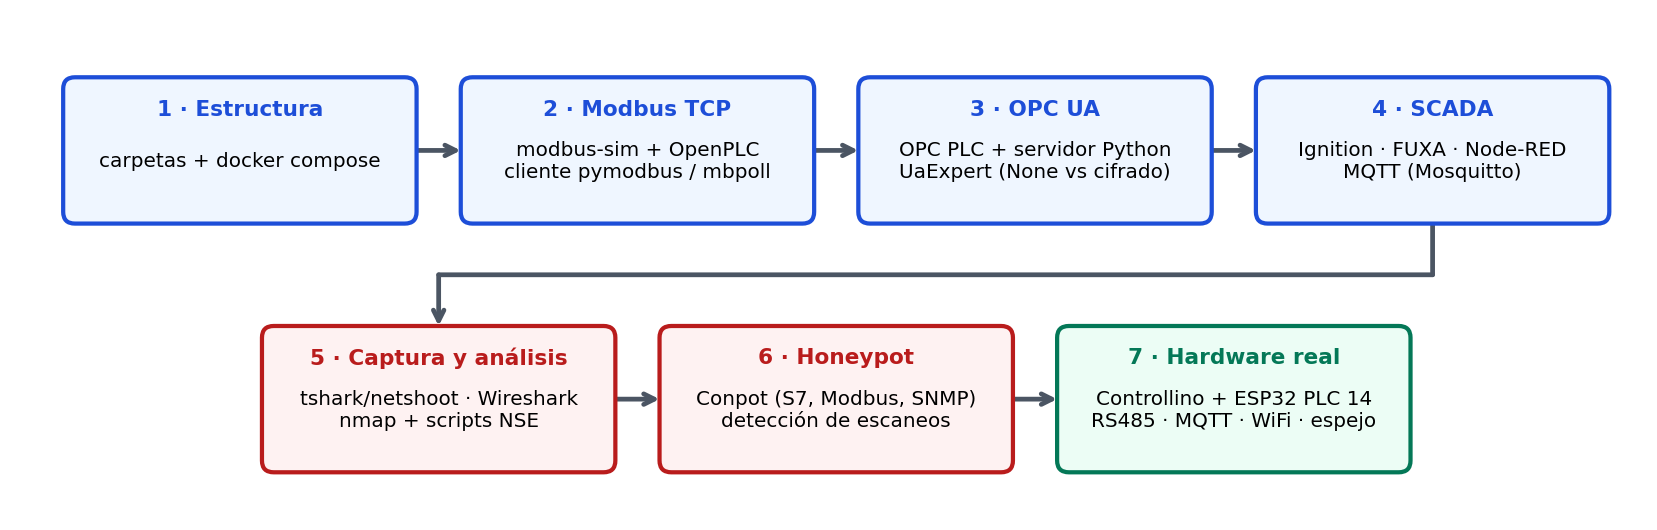
\includegraphics[width=\textwidth]{fig6_ruta}
  \caption{Orden de montaje del laboratorio: cada paso añade una capa sobre la anterior.}
  \label{fig:ruta}
\end{figure}

\section{Convenciones}

\begin{itemize}
  \item Los comandos se muestran en bloques de código; el símbolo \cmd{\$} no se escribe. Todos se ejecutan desde la carpeta \lab{} salvo indicación contraria.
  \item Las rutas de menú se escriben como \menu{Config \ra{} OPC UA \ra{} Connections}.
  \item Las direcciones IP de la red Docker son \ip{172.28.0.x}; las del segmento físico OT, \ip{192.168.10.x}. Desde el host (macOS o Windows) los servicios se alcanzan siempre por \ip{localhost:<puerto publicado>}.
  \item Las cajas de color destacan notas, avisos, errores críticos y resultados esperados.
\end{itemize}

\begin{nota}[Archivos de referencia]
Todo el laboratorio vive en la carpeta \lab{}. Los archivos íntegros (\cmd{docker-compose.yml}, \cmd{modbus/server.json}, \cmd{opcua/server.py}, \cmd{mosquitto/mosquitto.conf}) están reproducidos en el anexo~\ref{cap:anexos} y en la subcarpeta \cmd{docs/latex/src/} de esta guía.
\end{nota}

\chapter{Marco teórico}
\label{cap:teoria}

Este capítulo describe las tecnologías y herramientas que componen el laboratorio. Se agrupan siguiendo la pirámide de automatización: primero el modelo de referencia, luego la plataforma de contenedores que lo aloja, después los tres protocolos (Modbus, OPC~UA, MQTT), las herramientas de control y supervisión, las de análisis y seguridad y, por último, el hardware físico.

% -----------------------------------------------------------------------------
\section{Redes industriales y la pirámide de automatización}
\label{sec:piramide}

El modelo de referencia más usado para describir una planta es la \emph{pirámide de automatización} (ISA-95 / modelo de Purdue), que organiza los sistemas en niveles según su función y su horizonte temporal (figura~\ref{fig:niveles}). El \textbf{nivel~0} son sensores y actuadores; el \textbf{nivel~1}, los controladores (PLC, RTU) que ejecutan lazos en milisegundos; el \textbf{nivel~2}, la supervisión (SCADA/HMI, historiadores) que sondea a los controladores en el orden de segundos; el \textbf{nivel~3}, la gestión de operaciones (MES); y el \textbf{nivel~4}, los sistemas corporativos (ERP). Entre los niveles 3 y 4 la práctica moderna inserta una \emph{DMZ industrial} (nivel~3.5) que rompe la conectividad directa entre la red de planta (OT) y la red de empresa (IT).

\begin{figure}[H]
  \centering
  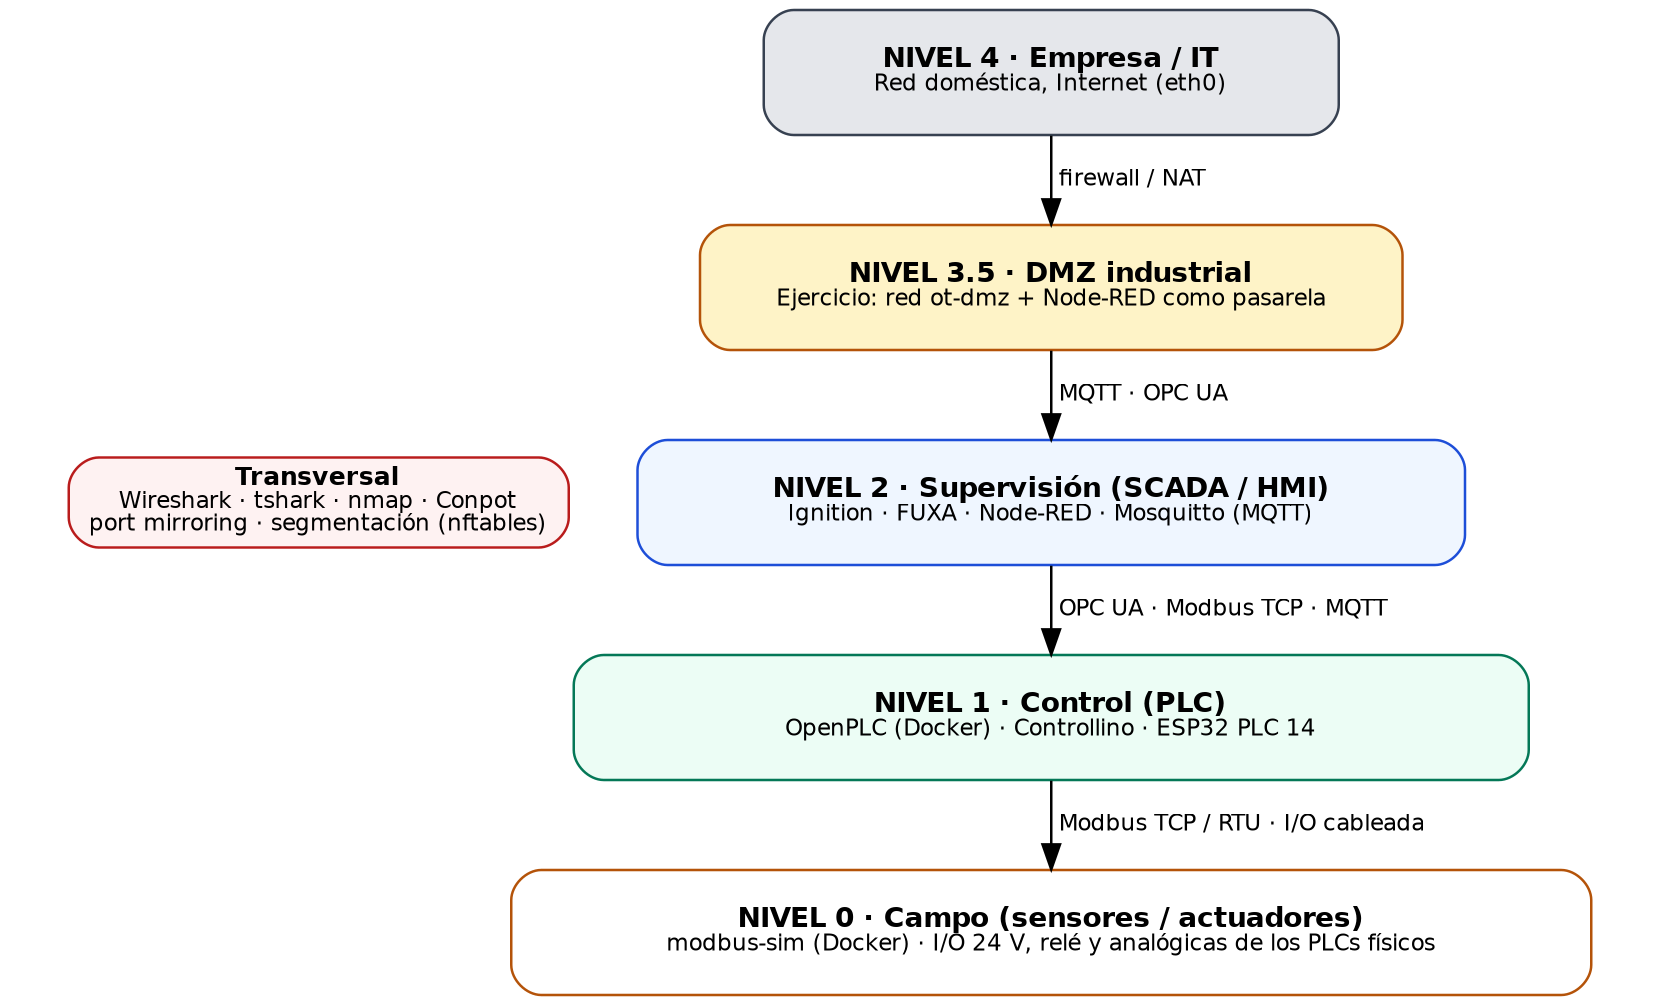
\includegraphics[width=0.95\textwidth]{fig2_niveles}
  \caption{Niveles de la pirámide de automatización y herramienta del laboratorio que ocupa cada uno.}
  \label{fig:niveles}
\end{figure}

Las redes OT difieren de las IT en varios aspectos que condicionan todo el laboratorio (tabla~\ref{tab:itot}). La prioridad es la disponibilidad y el determinismo, no la confidencialidad; los equipos viven décadas y rara vez se parchean; los protocolos nacieron sin autenticación porque asumían un cable aislado. Por eso el análisis de tráfico es tan revelador en OT: casi todo viaja en claro y es interpretable.

\begin{table}[H]
\centering\small
\caption{Diferencias entre redes IT y OT relevantes para el laboratorio.}
\label{tab:itot}
\begin{tabularx}{\textwidth}{L{3.2cm} X X}
\toprule
\textbf{Aspecto} & \textbf{Red IT} & \textbf{Red OT} \\
\midrule
Prioridad & Confidencialidad, integridad & Disponibilidad, seguridad física, determinismo \\
Patrón de tráfico & Ráfagas, cliente--servidor variado & Sondeo periódico (\emph{polling}) muy regular \\
Ciclo de vida & 3--5 años & 15--25 años \\
Autenticación & Habitual (TLS, Kerberos) & Ausente en Modbus, S7, EtherNet/IP clásico; opcional en OPC UA y MQTT \\
Latencia tolerable & Cientos de ms & De 1~ms (control de movimiento) a 1~s (supervisión) \\
Consecuencia de un fallo & Pérdida de datos & Parada de planta, daño físico \\
\bottomrule
\end{tabularx}
\end{table}

% -----------------------------------------------------------------------------
\section{Contenedores: Docker y Docker Compose}
\label{sec:docker}

\subsection{Conceptos}

Un \textbf{contenedor} es un proceso aislado del resto del sistema mediante \emph{namespaces} (PID, red, sistema de archivos) y \emph{cgroups} (límites de CPU y memoria) del kernel Linux. A diferencia de una máquina virtual no lleva su propio kernel, por lo que arranca en milisegundos y consume solo la memoria de la aplicación. Una \textbf{imagen} es la plantilla inmutable, construida por capas a partir de un \cmd{Dockerfile}, de la que se instancian contenedores. Un \textbf{registro} (Docker Hub, \cmd{mcr.microsoft.com}) almacena y distribuye imágenes.

\textbf{Docker Compose} describe en un archivo YAML un conjunto de servicios, redes y volúmenes y los gestiona como una unidad (\cmd{docker compose up/down/ps/logs}). En este laboratorio, \cmd{docker-compose.yml} define nueve servicios sobre una red común.

\subsection{Redes}

Docker crea por defecto redes de tipo \emph{bridge}: un conmutador virtual (en Linux, una interfaz \cmd{br-<id>}) al que se conecta la interfaz \cmd{eth0} de cada contenedor. Los contenedores de la misma red se ven entre sí por IP y por nombre de servicio (Docker incluye un DNS interno). Para que el host o el exterior alcancen un servicio se \emph{publica} un puerto (\cmd{"8088:8088"}), lo que instala una regla NAT del puerto del host al del contenedor. En el laboratorio asignamos IPs fijas (\cmd{ipv4\_address}) en la subred \ip{172.28.0.0/24} para que las capturas y los escaneos sean legibles y repetibles.

\begin{figure}[H]
\centering
\begin{tikzpicture}[node distance=6mm]
  % Linux
  \node[cajagris,minimum width=62mm,minimum height=56mm,anchor=north west] (hostL) at (0,0) {};
  \node[font=\small\bfseries,anchor=north west] at ($(hostL.north west)+(2mm,-1mm)$) {Host Linux};
  \node[caja,minimum width=50mm] (brL) at ($(hostL.north)+(0,-13mm)$) {bridge \cmd{br-xxxx} 172.28.0.1};
  \node[cajaverde,minimum width=14mm,font=\scriptsize] (c1) at ($(brL.south)+(-18mm,-11mm)$) {openplc\\.10};
  \node[cajaverde,minimum width=14mm,font=\scriptsize] (c2) at ($(brL.south)+(0,-11mm)$) {ignition\\.50};
  \node[cajaverde,minimum width=14mm,font=\scriptsize] (c3) at ($(brL.south)+(18mm,-11mm)$) {modbus-sim\\.30};
  \foreach \c in {c1,c2,c3} \draw[thick,azul] (\c.north) -- (brL.south -| \c.north);
  \node[cajaroja,text width=50mm,font=\scriptsize] (wsL) at ($(hostL.south)+(0,7mm)$) {Wireshark ve \cmd{br-xxxx} directamente};
  % macOS
  \node[cajagris,minimum width=62mm,minimum height=56mm,anchor=north west] (hostM) at (7.6,0) {};
  \node[font=\small\bfseries,anchor=north west] at ($(hostM.north west)+(2mm,-1mm)$) {Host macOS / Windows};
  \node[caja,draw=gris,dashed,minimum width=54mm,minimum height=30mm] (vm) at ($(hostM.north)+(0,-22mm)$) {};
  \node[font=\scriptsize,anchor=north west,gris] at ($(vm.north west)+(1mm,-0.5mm)$) {VM Linux oculta (Docker Desktop)};
  \node[caja,minimum width=44mm,font=\scriptsize] (brM) at ($(vm.north)+(0,-9mm)$) {bridge 172.28.0.0/24};
  \node[cajaverde,minimum width=12mm,font=\scriptsize] (m1) at ($(brM.south)+(-15mm,-8mm)$) {.10};
  \node[cajaverde,minimum width=12mm,font=\scriptsize] (m2) at ($(brM.south)+(0,-8mm)$) {.50};
  \node[cajaverde,minimum width=12mm,font=\scriptsize] (m3) at ($(brM.south)+(15mm,-8mm)$) {.30};
  \foreach \c in {m1,m2,m3} \draw[thick,azul] (\c.north) -- (brM.south -| \c.north);
  \node[cajanaranja,text width=54mm,font=\scriptsize] (natM) at ($(hostM.south)+(0,8mm)$) {Solo \cmd{localhost:<puerto>}; 172.28.0.x no es alcanzable desde el host};
  \draw[flechan] (natM.north) -- (vm.south);
\end{tikzpicture}
\caption{Red bridge de Docker en Linux frente a Docker Desktop (macOS/Windows). En Linux el bridge es una interfaz real del host; en macOS vive dentro de una máquina virtual y solo se accede por los puertos publicados.}
\label{fig:dockernet}
\end{figure}

\begin{aviso}[Implicación para macOS y Windows]
En Docker Desktop la red \ip{172.28.0.x} no es alcanzable desde el host y no existe una interfaz \cmd{br-xxxx} que Wireshark pueda abrir. Las capturas se hacen \emph{dentro} de la red Docker con un contenedor auxiliar (\cmd{netshoot}, sección~\ref{sec:netshoot}) o en el segmento físico. Entre contenedores las IPs fijas funcionan con normalidad.
\end{aviso}

\subsection{Volúmenes: bind mounts frente a volúmenes con nombre}
\label{sec:volumenes}

El sistema de archivos de un contenedor es efímero. Para persistir datos hay dos mecanismos que se comportan de forma distinta al arrancar sobre un directorio vacío, y esa diferencia fue la causa de uno de los fallos de la puesta en marcha (sección~\ref{sec:fallos}):

\begin{itemize}
  \item \textbf{Bind mount} (\cmd{./carpeta:/ruta}): monta una carpeta del host sobre la ruta del contenedor. Lo que hubiera en la imagen en esa ruta queda \emph{oculto}; si la carpeta del host está vacía, el contenedor ve un directorio vacío.
  \item \textbf{Volumen con nombre} (\cmd{nombre:/ruta}): gestionado por Docker. La primera vez que se monta vacío, Docker \emph{copia} en él el contenido que la imagen tenía en esa ruta. Es el mecanismo que esperan imágenes como Ignition, que traen un directorio \cmd{data/} preconfigurado.
\end{itemize}

\begin{figure}[H]
\centering
\begin{tikzpicture}
  \node[caja,minimum width=34mm] (img) at (0,0) {Imagen\\\cmd{/data} con archivos};
  \node[cajaroja,minimum width=40mm] (bind) at (5.2,1.1) {Bind mount vacío\\\cmd{/data} = \{\} (oculta la imagen)};
  \node[cajaverde,minimum width=40mm] (vol) at (5.2,-1.1) {Volumen con nombre vacío\\\cmd{/data} = copia de la imagen};
  \draw[flechar] (img.east) -- (bind.west) node[etiqueta,midway,above] {sin copia};
  \draw[flechav] (img.east) -- (vol.west) node[etiqueta,midway,below] {copia inicial};
\end{tikzpicture}
\caption{Comportamiento de Docker al montar un directorio vacío sobre una ruta que la imagen ya rellenaba.}
\label{fig:volumenes}
\end{figure}

\subsection{Arquitecturas de CPU e imágenes multi-arquitectura}

Una imagen contiene binarios compilados para una arquitectura. Los Mac con Apple Silicon (y la Raspberry Pi) son \cmd{arm64}; la mayoría de los PC, \cmd{amd64}. Muchas imágenes publican un \emph{manifiesto multi-arquitectura} y Docker escoge la variante adecuada. Cuando solo existe \cmd{amd64} (caso de \cmd{tuttas/openplc\_v3} y \cmd{honeynet/conpot}), en un Mac ARM hay que indicarlo con \cmd{platform: linux/amd64}: Docker Desktop la ejecuta mediante emulación (QEMU o Rosetta~2), más lenta pero funcional. Sin esa línea el error es \cmd{exec format error}.

% -----------------------------------------------------------------------------
\section{Modbus}
\label{sec:modbus}

\subsection{Origen y modelo}

Modbus (Modicon, 1979) es el protocolo industrial más extendido por su simplicidad y por ser de especificación abierta. Sigue un modelo \textbf{maestro--esclavo} (en la terminología actual, cliente--servidor): el maestro envía una petición y un único esclavo responde; los esclavos nunca hablan espontáneamente. Existen dos variantes principales:

\begin{itemize}
  \item \textbf{Modbus RTU}: sobre línea serie (habitualmente RS485 half-duplex, 9600--115200 bps, 8N1). Un bus multipunto con hasta 247 esclavos identificados por su \emph{unit ID}. La trama se delimita por silencios de al menos 3,5~caracteres y termina con un CRC-16.
  \item \textbf{Modbus TCP}: la misma PDU encapsulada en TCP (puerto 502) con una cabecera adicional, la \textbf{MBAP} (\emph{Modbus Application Protocol header}). Sin CRC (lo aporta TCP) y con un \emph{transaction ID} que permite peticiones concurrentes.
\end{itemize}

\subsection{Modelo de datos}

Un esclavo expone cuatro tablas (tabla~\ref{tab:modbustablas}). Las direcciones de protocolo van de 0 a 65535 en cada tabla. Históricamente se usaba una notación con prefijo (\emph{coils} 0xxxx, entradas discretas 1xxxx, registros de entrada 3xxxx, \emph{holding} 4xxxx, con base~1), de modo que ``40001'' significa \emph{holding register} de offset~0. Esta doble notación es fuente permanente de confusión y apareció en la puesta en marcha del simulador (sección~\ref{sec:fallos}): el archivo de configuración esperaba offsets de protocolo, no direcciones 4xxxx.

\begin{table}[H]
\centering\small
\caption{Tablas de datos Modbus y códigos de función asociados.}
\label{tab:modbustablas}
\begin{tabularx}{\textwidth}{L{3.4cm} L{1.5cm} L{1.6cm} L{2.6cm} X}
\toprule
\textbf{Tabla} & \textbf{Tamaño} & \textbf{Acceso} & \textbf{Notación 1-based} & \textbf{Funciones (FC)} \\
\midrule
Coils (salidas discretas) & 1 bit & R/W & 00001--09999 & 01 leer · 05 escribir uno · 15 escribir varios \\
Discrete inputs & 1 bit & R & 10001--19999 & 02 leer \\
Input registers & 16 bit & R & 30001--39999 & 04 leer \\
Holding registers & 16 bit & R/W & 40001--49999 & 03 leer · 06 escribir uno · 16 escribir varios · 23 leer/escribir \\
\bottomrule
\end{tabularx}
\end{table}

\subsection{Trama Modbus TCP}

La figura~\ref{fig:mbap} muestra la estructura de una petición Modbus TCP. La MBAP ocupa 7 bytes: \emph{transaction ID} (2), \emph{protocol ID} (2, siempre 0), \emph{length} (2, bytes que siguen) y \emph{unit ID} (1, dirección del esclavo, relevante en pasarelas TCP\ra{}RTU). Le sigue la PDU: código de función (1) y datos. En Wireshark el disector \cmd{mbtcp} muestra la MBAP y \cmd{modbus} la PDU, con los filtros \cmd{modbus.func\_code} y \cmd{modbus.exception\_code}.

\begin{figure}[H]
\centering
\begin{tikzpicture}[start chain=going right,node distance=0pt]
  \node[byte,fill=azulclaro,minimum width=19mm,on chain] (t) {Transaction ID\\2 bytes};
  \node[byte,fill=azulclaro,minimum width=17mm,on chain] (p) {Protocol ID\\2 bytes = 0};
  \node[byte,fill=azulclaro,minimum width=15mm,on chain] (l) {Length\\2 bytes};
  \node[byte,fill=azulclaro,minimum width=14mm,on chain] (u) {Unit ID\\1 byte};
  \node[byte,fill=verdeclaro,minimum width=17mm,on chain] (f) {Function\\1 byte};
  \node[byte,fill=verdeclaro,minimum width=20mm,on chain] (a) {Start addr.\\2 bytes};
  \node[byte,fill=verdeclaro,minimum width=18mm,on chain] (q) {Quantity\\2 bytes};
  \draw[decorate,decoration={brace,amplitude=4pt,mirror},azul] (t.south west) -- (u.south east) node[midway,below=5pt,font=\scriptsize,azul] {MBAP (7 bytes)};
  \draw[decorate,decoration={brace,amplitude=4pt,mirror},verde] (f.south west) -- (q.south east) node[midway,below=5pt,font=\scriptsize,verde] {PDU (FC 03: leer holding registers)};
  \node[font=\scriptsize,above=3pt of t.north west,anchor=south west] {Ejemplo: \cmd{00 01 | 00 00 | 00 06 | 01 | 03 | 00 00 | 00 03} $\Rightarrow$ leer 3 registros desde el offset 0 del esclavo 1};
\end{tikzpicture}
\caption{Estructura de una petición Modbus TCP: cabecera MBAP y PDU.}
\label{fig:mbap}
\end{figure}

Si la petición no puede atenderse, el esclavo responde con el código de función más 0x80 y un \emph{exception code} (01 función ilegal, 02 dirección ilegal, 03 valor ilegal, 04 fallo del dispositivo). Provocar una excepción leyendo un registro inexistente es uno de los primeros ejercicios de la guía.

\subsection{Seguridad}

Modbus carece de autenticación, autorización y cifrado: cualquier equipo con acceso a la red puede leer y escribir cualquier registro. Existe una variante Modbus/TCP Security (puerto 802, sobre TLS con certificados) con adopción muy escasa. En la práctica la protección viene de la red: segmentación, listas de acceso que solo permitan al SCADA hablar con los PLC y monitorización pasiva que alerte de escrituras (FC 05/06/15/16) desde orígenes no autorizados.

% -----------------------------------------------------------------------------
\section{OPC UA}
\label{sec:opcua}

\subsection{Qué resuelve}

OPC UA (IEC 62541, 2008) sustituye al OPC clásico basado en DCOM de Windows por un estándar independiente de plataforma para el intercambio de datos y metadatos en automatización. Frente a Modbus, aporta tres cosas: un \textbf{modelo de información} rico (los datos tienen nombre, tipo, unidades, jerarquía, no son registros anónimos), \textbf{servicios} de alto nivel (lectura, escritura, suscripción, métodos, alarmas, histórico) y \textbf{seguridad} integrada (certificados X.509, firma y cifrado, autenticación de usuario).

\subsection{Modelo de información}

Un servidor expone un \emph{espacio de direcciones} formado por nodos (objetos, variables, métodos, tipos) conectados por referencias. Cada nodo tiene un \emph{NodeId} (\cmd{ns=2;i=1001} o \cmd{ns=2;s=Tanque1.Nivel}) dentro de un \emph{namespace}. Los clientes navegan desde \cmd{Objects} igual que por un árbol de carpetas; UaExpert e Ignition lo hacen gráficamente. El servidor Python del laboratorio crea el objeto \cmd{Tanque1} con las variables \cmd{Nivel}, \cmd{Temperatura} y \cmd{Valvula} en el namespace \cmd{http://lab.local}.

\subsection{Pila de comunicaciones y seguridad}

La figura~\ref{fig:opcuapila} muestra la pila del transporte binario \cmd{opc.tcp} (puerto habitual 4840). Sobre TCP se establece un \textbf{SecureChannel} negociando una \emph{política de seguridad} (\cmd{None}, \cmd{Basic256Sha256}, \cmd{Aes256\_Sha256\_RsaPss}) y un \emph{modo} (\cmd{None}, \cmd{Sign}, \cmd{SignAndEncrypt}) mediante intercambio de certificados de aplicación. Dentro del canal se abre una \textbf{Session} donde el usuario se autentica (anónimo, usuario/contraseña o certificado). Solo entonces circulan los servicios (\cmd{Browse}, \cmd{Read}, \cmd{Write}, \cmd{CreateSubscription}, \cmd{Publish}).

\begin{figure}[H]
\centering
\begin{tikzpicture}
  \foreach \i/\txt/\col in {0/{Modelo de información: nodos, tipos, referencias (Tanque1.Nivel)}/verdeclaro,
                            1/{Servicios: Browse · Read · Write · Subscription/Publish · Call}/verdeclaro,
                            2/{Session: autenticación de usuario (anónimo, usuario/clave, certificado)}/azulclaro,
                            3/{SecureChannel: política (None, Basic256Sha256) + modo (None, Sign, SignAndEncrypt)}/azulclaro,
                            4/{UA TCP: Hello/Acknowledge, chunking de mensajes}/grisclaro,
                            5/{TCP/IP (puerto 4840, 50000, 62541)}/grisclaro}{
    \node[draw,fill=\col,minimum width=120mm,text width=116mm,align=center,minimum height=8mm,font=\small,rounded corners=2pt] at (0,-\i*9mm) {\txt};
  }
  \draw[decorate,decoration={brace,amplitude=5pt},thick,rojo] (6.3,0.4) -- (6.3,-2.7) node[midway,right=6pt,font=\scriptsize,align=left,rojo] {Visible en claro solo\\con None/None};
  \draw[decorate,decoration={brace,amplitude=5pt},thick,gris] (6.3,-3.2) -- (6.3,-4.9) node[midway,right=6pt,font=\scriptsize,align=left,gris] {Siempre visible\\(endpoints, certificados)};
\end{tikzpicture}
\caption{Pila OPC UA sobre transporte binario. El contraste entre una sesión \cmd{None/None} y una \cmd{SignAndEncrypt} es el ejercicio central de OPC UA en el laboratorio.}
\label{fig:opcuapila}
\end{figure}

\subsection{Descubrimiento y endpoints}

Un cliente primero pide al servidor sus \emph{endpoints} (\cmd{GetEndpoints}): la lista de combinaciones URL, política y modo que acepta. Esa respuesta viaja siempre en claro, por lo que un escáner puede saber qué políticas ofrece un servidor sin autenticarse. El servidor OPC PLC de Microsoft acepta cualquier certificado de cliente si se lanza con \cmd{--autoaccept}; en producción el administrador debe mover manualmente cada certificado de cliente a la lista de confianza.

% -----------------------------------------------------------------------------
\section{MQTT}
\label{sec:mqtt}

MQTT (1999, hoy estándar OASIS/ISO 20922) es un protocolo ligero de \textbf{publicación--suscripción} pensado para enlaces poco fiables. A diferencia de Modbus y OPC UA, no hay conexión directa entre productor y consumidor: ambos se conectan a un \textbf{broker} (Mosquitto en el laboratorio, puerto 1883; 8883 con TLS). Los publicadores envían mensajes a un \emph{topic} jerárquico (\cmd{ot/esp32/nivel}) y el broker los reenvía a quien esté suscrito, con comodines \cmd{+} (un nivel) y \cmd{\#} (todo lo que sigue). Tres niveles de QoS regulan la entrega (0: a lo sumo una vez; 1: al menos una vez; 2: exactamente una vez), y los mensajes \emph{retained} permiten que un nuevo suscriptor reciba el último valor al conectarse.

\begin{figure}[H]
\centering
\begin{tikzpicture}
  \node[cajaverde,minimum width=30mm] (esp) at (0,0) {ESP32 PLC 14\\publica \cmd{ot/esp32/nivel}};
  \node[caja,minimum width=30mm,fill=azulclaro] (broker) at (6.2,0) {Mosquitto\\broker :1883};
  \node[caja,minimum width=28mm] (nr) at (12.4,1.2) {Node-RED\\suscrito \cmd{ot/esp32/\#}};
  \node[caja,minimum width=28mm] (ign) at (12.4,-1.2) {Ignition MQTT Engine\\suscrito \cmd{ot/\#}};
  \draw[flechav] (esp) -- (broker) node[etiqueta,midway,above] {PUBLISH QoS 0};
  \draw[flecha] (broker) -- (nr);
  \draw[flecha] (broker) -- (ign);
  \draw[flechan] (nr.south west) to[bend left=20] node[etiqueta,pos=0.5,above=3pt] {\cmd{ot/esp32/cmd}} (broker.north east);
\end{tikzpicture}
\caption{Modelo publicación--suscripción de MQTT en el laboratorio.}
\label{fig:mqtt}
\end{figure}

En planta MQTT se usa como capa IIoT (Sparkplug~B define una carga útil y una semántica de estado para ello). Sin TLS, todo el payload es legible en Wireshark con el filtro \cmd{mqtt}; el ejercicio del capítulo~\ref{cap:ejercicios} compara 1883 con 8883.

% -----------------------------------------------------------------------------
\section{Herramientas de control (nivel 1)}
\label{sec:control}

\subsection{OpenPLC}

OpenPLC es un runtime de PLC de código abierto conforme a IEC 61131-3 (lenguajes LD, FBD, ST, IL, SFC). Se compone del \textbf{OpenPLC Editor} (herramienta de escritorio basada en Beremiz para escribir y compilar programas) y del \textbf{OpenPLC Runtime}, que ejecuta el programa compilado y expone una interfaz web (puerto 8080) para cargarlo, arrancarlo y configurar comunicaciones. El runtime actúa como \textbf{esclavo Modbus TCP} (puerto 502) publicando sus variables en las direcciones IEC (\cmd{\%IX0.0} entradas digitales, \cmd{\%QX0.0} salidas, \cmd{\%IW100} registros de entrada, \cmd{\%QW100} \emph{holding}), y también como \textbf{maestro} (menú \menu{Slave Devices}) que sondea otros esclavos Modbus y mapea sus registros en las mismas direcciones. Esa doble función es lo que permite que el PLC virtual en Docker lea el simulador y controle los PLC físicos. El Editor, además, compila programas para placas Arduino, Controllino y ESP32 dejándolas como esclavos Modbus TCP/RTU.

\subsection{OPC PLC (Microsoft)}

\cmd{mcr.microsoft.com/iotedge/opc-plc} es un servidor OPC UA de simulación creado para probar Azure IoT. Genera nodos con distintos comportamientos configurables por línea de comandos: \cmd{--sn} nodos lentos, \cmd{--fn} rápidos, \cmd{--gn} con ``fallos'' (picos, valores fuera de rango), \cmd{--sph} publica su propio certificado. Las opciones \cmd{--autoaccept}, \cmd{--ut} (usuarios anónimos) y \cmd{--dca} (no comprobar el dominio del certificado) relajan la seguridad para laboratorio y deben retirarse para practicar certificados. Escucha en el puerto 50000.

\subsection{Servidor OPC UA en Python (asyncua)}

\cmd{asyncua} (\emph{opcua-asyncio}) es la biblioteca Python de referencia para clientes y servidores OPC UA. El servidor del laboratorio (\cmd{opcua/server.py}, anexo~\ref{sec:anexo-opcua}) tiene 25 líneas: registra un namespace, crea un objeto con tres variables y actualiza dos de ellas cada segundo con funciones senoidales. Su valor didáctico es doble: muestra cómo se construye un espacio de direcciones y proporciona un servidor cuyo código se puede modificar (añadir métodos, exigir seguridad, cambiar tipos) para observar el efecto en la red.

% -----------------------------------------------------------------------------
\section{Herramientas de supervisión (nivel 2)}
\label{sec:scada}

\subsection{Ignition}

Ignition (Inductive Automation) es una plataforma SCADA/IIoT comercial basada en Java con arquitectura cliente--servidor centrada en el \textbf{Gateway} (figura~\ref{fig:ignition}). El Gateway es un único proceso que integra los \emph{drivers} de dispositivos (Modbus TCP, Siemens S7, Allen-Bradley Logix, Omron, DNP3, BACnet), un cliente y un servidor OPC UA, el sistema de \emph{tags}, el historiador (sobre una base de datos SQL), alarmas, scripting Python (Jython) y los módulos de visualización. Todo se administra por web (puerto 8088). El \textbf{Designer} es la herramienta de desarrollo, que se lanza desde el Gateway mediante el \emph{Designer Launcher}. \textbf{Perspective} es el módulo de HMI web (HTML5, responsive) y \textbf{Vision} el módulo clásico de cliente Java de escritorio.

\begin{figure}[H]
\centering
\begin{tikzpicture}
  \node[cajagris,minimum width=140mm,minimum height=44mm] (gw) at (0,0) {};
  \node[font=\small\bfseries,anchor=north west] at ($(gw.north west)+(2mm,-1mm)$) {Ignition Gateway (contenedor, :8088)};
  \node[caja,text width=28mm,font=\scriptsize] (drv) at (-5.1,0.6) {Drivers\\Modbus TCP · S7 · Logix};
  \node[caja,text width=28mm,font=\scriptsize] (opc) at (-1.7,0.6) {OPC UA\\cliente + servidor :62541};
  \node[caja,text width=28mm,font=\scriptsize] (mqtt) at (1.7,0.6) {MQTT Engine\\(módulo Cirrus Link)};
  \node[caja,text width=28mm,font=\scriptsize] (tags) at (5.1,0.6) {Tags · Historian\\Alarmas · Scripting};
  \node[caja,fill=azulclaro,minimum width=132mm,font=\scriptsize] (persp) at (0,-1.1) {Perspective (HMI web) · Vision · Reporting · Web Dev};
  \node[cajaverde,text width=26mm,font=\scriptsize] (plc) at (-5.1,-3.6) {OpenPLC\\Controllino · ESP32};
  \node[cajaverde,text width=26mm,font=\scriptsize] (srv) at (-1.7,-3.6) {OPC PLC\\opcua-py};
  \node[cajaverde,text width=26mm,font=\scriptsize] (mq) at (1.7,-3.6) {Mosquitto};
  \node[cajanaranja,text width=26mm,font=\scriptsize] (des) at (5.1,-3.6) {Designer Launcher\\navegador (sesiones)};
  \draw[flecha] (plc) -- (drv);
  \draw[flecha] (srv) -- (opc);
  \draw[flecha] (mq) -- (mqtt);
  \draw[flechan] (des) -- (persp.south -| des);
\end{tikzpicture}
\caption{Arquitectura de Ignition: un Gateway concentra drivers, OPC UA, tags y módulos de visualización; el Designer y las sesiones Perspective son clientes del Gateway.}
\label{fig:ignition}
\end{figure}

Ignition es relevante en un curso de redes porque su comportamiento es el de un SCADA de planta real: abre varias conexiones TCP por dispositivo, sondea a intervalos configurables (\emph{scan class} / \emph{tag group}), reintenta ante fallos y genera la ``firma'' de tráfico periódico que un analista debe reconocer. Su modelo de licencias se trata en el capítulo~\ref{cap:licencias}.

\subsection{FUXA}

FUXA es un SCADA/HMI web de código abierto (Node.js + Angular) mucho más ligero que Ignition. Ofrece conexiones Modbus TCP/RTU, OPC UA, S7, MQTT, BACnet y WebAPI, un editor gráfico de sinópticos SVG en el navegador (puerto 1881), alarmas y un histórico sencillo. Sirve como segundo cliente para contrastar cómo dos SCADA distintos sondean el mismo esclavo (número de conexiones, intervalo, agrupación de registros) y como alternativa cuando Ignition no está disponible.

\subsection{Node-RED}

Node-RED es un entorno de programación por flujos (nodos conectados en un editor web, puerto 1880) construido sobre Node.js. Con los paquetes \cmd{node-red-contrib-modbus} y \cmd{node-red-contrib-opcua} se convierte en una pasarela de protocolos: puede leer Modbus y publicar en MQTT, exponer un servidor OPC UA, o generar tráfico sintético continuo para capturar. En el laboratorio ocupa el papel de la ``pasarela'' en el ejercicio de DMZ y de consumidor MQTT del ESP32.

% -----------------------------------------------------------------------------
\section{Herramientas de análisis y seguridad}
\label{sec:analisis}

\subsection{Wireshark, tshark y tcpdump}

Wireshark es el analizador de protocolos de referencia; \cmd{tshark} es su versión de línea de comandos y \cmd{tcpdump} la utilidad clásica de captura a archivo \cmd{.pcap}. Wireshark incluye disectores para todos los protocolos del laboratorio: \cmd{mbtcp}/\cmd{modbus}, \cmd{opcua}, \cmd{mqtt}, \cmd{s7comm}, \cmd{enip}/\cmd{cip}, \cmd{pn\_io}/\cmd{pn\_dcp}. Dos herramientas de Wireshark son especialmente útiles en OT: \menu{Statistics \ra{} Conversations}, que resume quién habla con quién y cuánto, y \menu{Statistics \ra{} I/O Graph}, que muestra paquetes por segundo y revela la periodicidad del sondeo. Cuando un protocolo va por un puerto no estándar (OPC UA en 50000), se indica con \menu{Analyze \ra{} Decode As}.

\subsection{netshoot}
\label{sec:netshoot}

\cmd{nicolaka/netshoot} es una imagen Docker con decenas de herramientas de red (tshark, tcpdump, nmap, iperf, socat, dig\ldots). Su uso más potente es \cmd{docker run --net container:<nombre>}: el contenedor auxiliar se une al \emph{namespace de red} del contenedor objetivo y comparte su \cmd{eth0}, de modo que \cmd{tshark -i eth0} captura exactamente lo que ese servicio envía y recibe, sin tocar el host. Funciona igual en Linux, macOS y Windows, por lo que es el método de captura principal de esta guía.

\subsection{nmap y scripts NSE}

nmap descubre hosts y puertos; con el \emph{Nmap Scripting Engine} incorpora scripts específicos de ICS: \cmd{modbus-discover} (identifica esclavos y lee su ID de dispositivo), \cmd{s7-info} (extrae modelo, firmware y número de serie de un S7 vía S7comm), \cmd{enip-info}, \cmd{bacnet-info}. El escaneo es la primera fase de cualquier intrusión y también la forma de inventariar una red propia; en OT debe hacerse con cuidado porque algunos PLC antiguos se bloquean ante escaneos agresivos.

\subsection{Conpot}

Conpot (proyecto Honeynet) es un \textbf{honeypot} de sistemas de control: un servidor que imita un PLC (por defecto un Siemens S7-300 con S7comm en el 102, Modbus en el 502, SNMP en el 161 y una web de diagnóstico en el 80) y registra en detalle cada conexión. Desplegado en una red real, cualquier tráfico que reciba es por definición sospechoso, porque ningún proceso legítimo lo necesita. En el laboratorio sirve para ver cómo ``luce'' un PLC ante nmap y para correlacionar un escaneo con el log del honeypot, que es el principio de la detección de intrusos en OT.

\subsection{UaExpert}

UaExpert (Unified Automation) es el cliente OPC UA gráfico de referencia, gratuito con registro. Permite descubrir endpoints, elegir política y modo de seguridad, gestionar certificados, navegar el espacio de direcciones, leer, escribir, suscribirse y llamar métodos. Es la forma más rápida de comparar una conexión sin seguridad con una cifrada.

\subsection{Monitorización pasiva y port mirroring}

Los sensores de red OT comerciales (Nozomi, Claroty, Dragos) y los de código abierto (Zeek, Suricata con reglas Modbus) no se instalan en los PLC: escuchan una copia del tráfico obtenida de un puerto espejo (\emph{SPAN/mirror}) del switch o de un TAP. El laboratorio reproduce esa posición con un switch gestionable barato cuyo puerto espejo alimenta una NIC de captura del host (figura~\ref{fig:captura}). La lección es que la visibilidad de la red depende de dónde se coloque el sensor, no solo de la herramienta.

\begin{figure}[H]
  \centering
  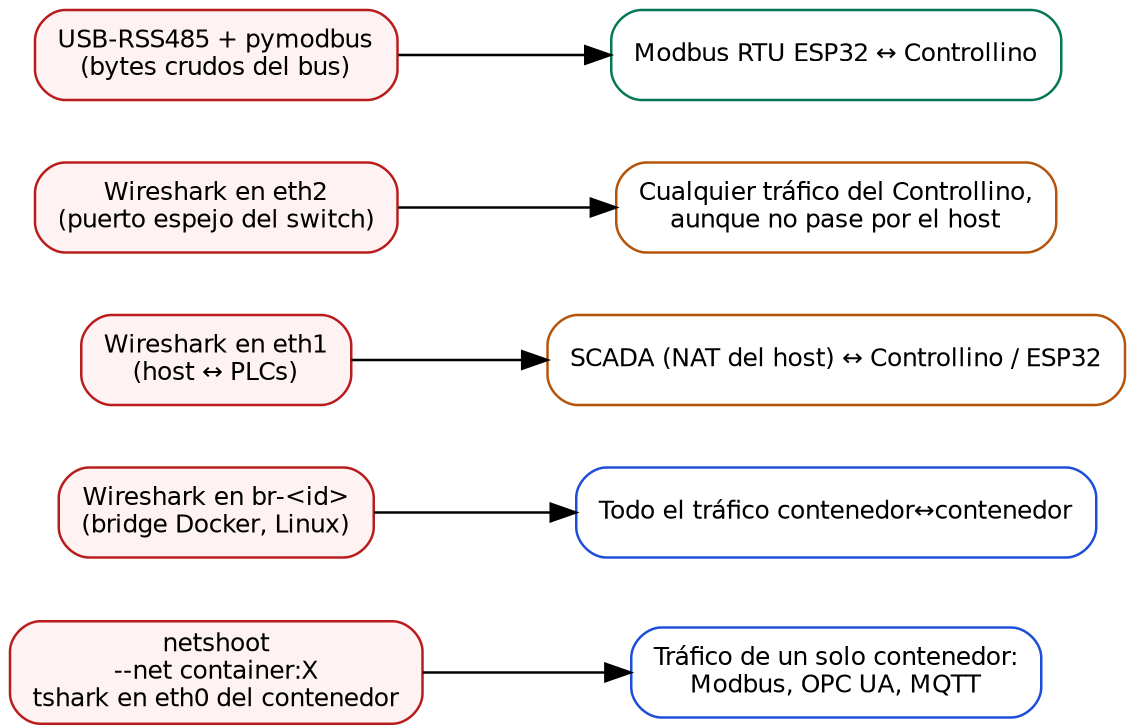
\includegraphics[width=0.9\textwidth]{fig5_captura}
  \caption{Puntos de captura del laboratorio y qué tráfico se observa en cada uno.}
  \label{fig:captura}
\end{figure}

% -----------------------------------------------------------------------------
\section{Hardware físico}
\label{sec:hardware}

\subsection{Controllino}

Controllino es una familia de PLC industriales basados en Arduino (ATmega328 en el MINI; ATmega2560 en MAXI y MEGA) con entradas y salidas a 24~V, relés, RTC y, en los modelos MAXI/MEGA, Ethernet 10/100 (controlador Wiznet W5100) y RS485. Se programa con el Arduino IDE y las librerías estándar (\cmd{Ethernet}, \cmd{ArduinoModbus}, \cmd{ArduinoRS485}), o con OpenPLC Editor en IEC 61131-3. Sus limitaciones son didácticamente valiosas: el W5100 admite solo 4 sockets simultáneos y el microcontrolador a 16~MHz responde a Modbus con una latencia claramente mayor que la de un simulador, lo que se mide en Wireshark.

\subsection{ESP32 PLC 14 (Industrial Shields)}

El ESP32 PLC~14 lleva un ESP32 de doble núcleo a 240~MHz con WiFi y Bluetooth, Ethernet RJ45, RS485 half-duplex, I2C de expansión, RTC, entradas analógicas 0--10~V / 4--20~mA y un relé. Industrial Shields proporciona el paquete de placas \cmd{industrialshields-esp32} y la librería \textbf{Tools40} con clases Modbus TCP/RTU maestro y esclavo. Su potencia y su doble conectividad (cable y WiFi) lo hacen ideal para tres papeles: esclavo Modbus TCP, \textbf{pasarela RTU\ra{}TCP} que expone al Controllino por Ethernet, y publicador MQTT.

\subsection{RS485 y Modbus RTU}

RS485 es una capa física serie diferencial (par A/B) multipunto y half-duplex, con alcance de hasta 1200~m y hasta 32 nodos por segmento sin repetidores. Requiere terminación de 120~$\Omega$ en ambos extremos y una referencia de masa común. Sobre ella corre Modbus RTU, donde el tiempo de silencio entre tramas es parte del protocolo: un analizador debe capturar los bytes crudos (adaptador USB-RS485 en paralelo al bus) y reconstruir las tramas por tiempo o por CRC. Wireshark no lee puertos serie directamente, pero un volcado se puede encapsular con \cmd{socat} y decodificar como \cmd{mbrtu}.

% -----------------------------------------------------------------------------
\section{Ethernet industrial en tiempo real}
\label{sec:rt}

PROFINET, EtherNet/IP con I/O implícito y EtherCAT trabajan en capa~2: usan tramas Ethernet propias (EtherType específico), multicast y tiempos de ciclo del orden de milisegundos. El bridge de Docker es una abstracción de capa~3 y en macOS/Windows ni siquiera expone la NIC real, por lo que estos protocolos no se simulan bien en contenedores. La tabla~\ref{tab:rt} resume las opciones si se quieren añadir al laboratorio.

\begin{table}[H]
\centering\small
\caption{Opciones para estudiar Ethernet industrial de tiempo real fuera de Docker.}
\label{tab:rt}
\begin{tabularx}{\textwidth}{L{2.6cm} L{4.6cm} X}
\toprule
\textbf{Protocolo} & \textbf{Opción recomendada} & \textbf{Notas} \\
\midrule
PROFINET (controlador) & TIA Portal + PLCSIM Advanced (Windows, trial) & Expone un controlador PROFINET virtual sobre la NIC del PC; filtro \cmd{pn\_dcp} para ver el descubrimiento. \\
PROFINET (dispositivo) & p-net (RT-Labs) en Raspberry Pi o VM Linux & Puede correr en contenedor solo en Linux nativo con \cmd{network\_mode: host} y \cmd{cap\_add: NET\_ADMIN, NET\_RAW}. \\
EtherNet/IP & OpENer (adaptador open source) o driver de Ignition contra un PLC real & OpENer funciona en contenedor Linux con \cmd{network\_mode: host}. \\
EtherCAT & SOEM + un esclavo real (p.\,ej. Beckhoff EL1008 usado) & No existe simulador serio sin hardware. \\
\bottomrule
\end{tabularx}
\end{table}

Con el Controllino y el ESP32 se cubren Modbus TCP/RTU y MQTT sobre hardware real; un S7-1200 o un Micro820 de segunda mano completan el laboratorio para PROFINET y EtherNet/IP.

\chapter{Licencias y costes}
\label{cap:licencias}

Casi todo el laboratorio es software libre o gratuito. Las excepciones relevantes son Ignition, cuyo modelo conviene entender antes de usarlo en clase, y algunas herramientas de escritorio que exigen registro. La tabla~\ref{tab:licencias} resume la situación; las secciones siguientes detallan los casos con matices.

\begin{table}[H]
\centering\small
\caption{Licencia y coste de cada componente del laboratorio.}
\label{tab:licencias}
\begin{tabularx}{\textwidth}{L{3.6cm} L{3.4cm} X}
\toprule
\textbf{Componente} & \textbf{Licencia} & \textbf{Coste y condiciones} \\
\midrule
Docker Engine (Linux) & Apache 2.0 & Gratuito. \\
Docker Desktop (macOS/Win) & Propietaria (Docker Subscription Service Agreement) & Gratuito para uso personal, educativo, proyectos de código abierto y empresas pequeñas; las grandes empresas requieren suscripción. Uso académico cubierto. \\
OpenPLC Runtime y Editor & GPLv3 & Gratuito. \\
\cmd{oitc/modbus-server} & Código abierto & Gratuito. \\
OPC PLC (Microsoft) & MIT & Gratuito. \\
asyncua (opcua-asyncio) & LGPL-3.0 & Gratuito. \\
Ignition & Propietaria & \textbf{Trial gratuito ilimitado} en bloques de 2~h reiniciables; \textbf{Maker Edition} gratuita para uso personal/educativo no comercial; licencia comercial perpetua por servidor. Ver sección~\ref{sec:lic-ignition}. \\
FUXA & MIT & Gratuito. \\
Node-RED & Apache 2.0 & Gratuito. \\
Eclipse Mosquitto & EPL-2.0 / EDL-1.0 & Gratuito. \\
Conpot & GPLv2 & Gratuito. \\
netshoot, nmap, tcpdump & Código abierto (nmap: NPSL) & Gratuito. \\
Wireshark & GPLv2 & Gratuito. \\
UaExpert & Propietaria & Gratuito para uso no comercial; requiere registro en \url{unified-automation.com} para descargar. \\
Arduino IDE & AGPL-3.0 / GPL & Gratuito. \\
Tools40 (Industrial Shields) & LGPL & Gratuito. \\
Factory I/O (opcional) & Propietaria & Simulador 3D de planta con Modbus/OPC UA. Versión de prueba de 30~días; licencias de pago con descuento educativo. Solo Windows. \\
\bottomrule
\end{tabularx}
\end{table}

% -----------------------------------------------------------------------------
\section{Ignition}
\label{sec:lic-ignition}

Ignition no exige pago para usarse en laboratorio. Existen tres vías, resumidas en la figura~\ref{fig:lic-ignition}.

\subsection{Modo trial (edición Standard)}

Al instalar Ignition sin licencia, \emph{todos} los módulos funcionan de forma completa durante 2~horas. Al expirar, los módulos se detienen (el Gateway sigue vivo) y en la cabecera de la web aparece \menu{Reset Trial}: un clic reinicia el contador otras 2~horas, sin límite de repeticiones, sin cuenta y sin conexión a Internet. Es el modo que usa el \cmd{docker-compose.yml} del laboratorio (\cmd{IGNITION\_EDITION: "standard"}) y el recomendado para las sesiones de clase, porque no impone restricciones de módulos y no depende de licencias externas. El único inconveniente es tener que pulsar \menu{Reset Trial} en sesiones largas.

\subsection{Maker Edition}

Maker Edition es una licencia gratuita permanente destinada a uso \textbf{personal y educativo no comercial}. Se obtiene creando una cuenta en \url{account.inductiveautomation.com}, que entrega una clave de licencia y un token de activación; en Docker se pasan como \cmd{IGNITION\_EDITION: "maker"}, \cmd{IGNITION\_LICENSE\_KEY} e \cmd{IGNITION\_ACTIVATION\_TOKEN}. El Gateway debe poder contactar periódicamente con \cmd{licensing.inductiveautomation.com} (HTTPS); si pierde la conexión durante un tiempo vuelve al modo trial.

Sus limitaciones respecto a Standard son: máximo 10 sesiones Perspective simultáneas, 10\,000 tags, sin Perspective Workstation (aplicación de escritorio), sin Vision (cliente Java clásico) y redundancia solo en modo independiente. Incluye los módulos que el laboratorio necesita: driver Modbus TCP, OPC UA (cliente y servidor), Perspective, Historian, Alarm Notification, Reporting, SQL Bridge, SFC, Serial Support, UDP/TCP Driver, Web Dev y los drivers Siemens, Allen-Bradley y Omron. Los módulos MQTT de Cirrus Link (MQTT Engine, Transmission, Distributor) son de terceros y están habilitados para Maker. En resumen, \textbf{no quita nada relevante para trabajar con Controllino, ESP32, OpenPLC ni con los servidores OPC UA del laboratorio}.

\subsection{Licencias educativas y comerciales}

La documentación de Maker indica que para instituciones educativas (aulas, proyectos de fin de carrera) Inductive Automation ofrece opciones específicas a través de su equipo de ventas. Para un uso formal en la Universidad de Cuenca lo correcto es solicitar esa licencia educativa. La licencia comercial es perpetua por servidor (no una suscripción) y solo tiene sentido en producción.

\begin{figure}[H]
\centering
\begin{tikzpicture}[font=\footnotesize]
  \node[caja,fill=azulclaro,text width=40mm] (q1) at (0,0) {¿Sesiones de clase de pocas horas o uso puntual?};
  \node[cajaverde,text width=38mm] (trial) at (-3.4,-2.3) {\textbf{Trial Standard}\\2 h reiniciables, sin cuenta, sin Internet, todos los módulos};
  \node[caja,fill=azulclaro,text width=38mm] (q2) at (3.4,-2.3) {¿Gateway encendido días sin intervención?};
  \node[cajaverde,text width=38mm] (maker) at (1.0,-4.9) {\textbf{Maker Edition}\\gratuita, cuenta IA, Internet, 10 sesiones / 10\,000 tags};
  \node[cajanaranja,text width=38mm] (edu) at (5.8,-4.9) {\textbf{Licencia educativa}\\solicitar a ventas de IA (uso institucional)};
  \draw[flecha] (q1) -- node[etiqueta,above left] {sí} (trial);
  \draw[flecha] (q1) -- node[etiqueta,above right] {no} (q2);
  \draw[flecha] (q2) -- node[etiqueta,above left] {personal} (maker);
  \draw[flecha] (q2) -- node[etiqueta,above right] {institucional} (edu);
\end{tikzpicture}
\caption{Elección de la vía de licenciamiento de Ignition para el laboratorio.}
\label{fig:lic-ignition}
\end{figure}

\begin{nota}[Recomendación adoptada]
El laboratorio se despliega en modo \textbf{trial Standard}. Si se quiere un Gateway permanente para demostraciones, cambiar a Maker es un cambio de tres variables de entorno en el \cmd{docker-compose.yml}; el proyecto y los tags se conservan en el volumen \cmd{ignition-data}.
\end{nota}

% -----------------------------------------------------------------------------
\section{Docker Desktop}

Docker Engine en Linux es software libre sin restricciones. Docker Desktop (el paquete gráfico para macOS y Windows que incluye la máquina virtual, Compose y Kubernetes) es gratuito para uso personal, educativo y de código abierto, y para empresas de menos de 250 empleados y menos de 10~millones de dólares de facturación; por encima de ese umbral requiere una suscripción de pago. El uso académico en la universidad está cubierto por la modalidad gratuita.

% -----------------------------------------------------------------------------
\section{UaExpert y otras herramientas de escritorio}

UaExpert se descarga gratis tras registrarse en la web de Unified Automation; la licencia permite uso no comercial y evaluación. No hay límite temporal. Wireshark, nmap, Arduino IDE y OpenPLC Editor son software libre. Factory I/O, cuyo instalador está en la carpeta del curso, es un simulador 3D de planta (Windows) que se comunica por Modbus TCP y OPC UA y puede sustituir al \cmd{modbus-sim} como ``proceso'' visual; su versión de prueba dura 30~días y las licencias educativas son de pago con descuento. Es opcional y no forma parte de las prácticas de esta guía.

\chapter{Instalación y puesta en marcha}
\label{cap:instalacion}

Este capítulo lleva desde un equipo sin nada instalado hasta los nueve contenedores en marcha y verificados. Recoge además los cuatro problemas que aparecieron al desplegar el laboratorio en macOS y cómo se resolvieron, porque cada uno ilustra un concepto de Docker que conviene conocer.

% -----------------------------------------------------------------------------
\section{Requisitos}

\begin{table}[H]
\centering\small
\caption{Requisitos de software y hardware.}
\label{tab:requisitos}
\begin{tabularx}{\textwidth}{L{5.2cm} L{2.6cm} X}
\toprule
\textbf{Herramienta} & \textbf{Dónde corre} & \textbf{Para qué} \\
\midrule
Docker Engine + Compose v2 (Linux) o Docker Desktop (macOS/Windows) & Host & Toda la infraestructura \\
Wireshark & Host & Analizar capturas \\
UaExpert & Host & Cliente OPC UA gráfico \\
Python 3.10+ con \cmd{pymodbus} y \cmd{asyncua} (opcional) & Host & Scripts propios; todo puede hacerse también desde contenedores \\
Arduino IDE 1.8.x/2.x + paquete \cmd{industrialshields-esp32} + placas Controllino & Host & Firmware de los PLC físicos \\
OpenPLC Editor & Host & Programar en IEC 61131-3 y subir firmware Modbus a las placas \\
Switch Ethernet, idealmente gestionable con \emph{port mirroring} (p.\,ej. TP-Link TL-SG105E) & Físico & Segmento OT real y captura entre PLC \\
Adaptador USB-Ethernet (segunda NIC) y adaptador USB-RS485 & Físico & Segmento OT aislado y análisis de Modbus RTU \\
Fuente 24~Vdc $\geq$ 2~A & Físico & Alimentar ambos PLC (no solo por USB) \\
\bottomrule
\end{tabularx}
\end{table}

Recursos mínimos del host: 8~GB de RAM (Ignition consume 1--2~GB; en macOS asigne al menos 6~GB a Docker Desktop), 15~GB de disco para imágenes y conexión a Internet para la primera descarga (la imagen de Ignition supera 1~GB).

% -----------------------------------------------------------------------------
\section{Elección de plataforma}
\label{sec:plataforma}

El laboratorio funciona en Linux, macOS y Windows, pero no de forma idéntica (sección~\ref{sec:docker}). En \textbf{Linux nativo} el bridge de Docker es una interfaz visible en Wireshark, se puede usar \cmd{network\_mode: host} y macvlan, y el host alcanza las IPs \ip{172.28.0.x}. En \textbf{macOS y Windows} Docker Desktop ejecuta los contenedores dentro de una VM: se trabaja por puertos publicados y se captura desde dentro con netshoot. Ambas vías cubren todas las prácticas; la de Linux ofrece más puntos de captura.

\begin{nota}[Recomendación]
Para un curso, la combinación más cómoda es Docker Desktop en el portátil de cada estudiante (macOS/Windows) para las prácticas de protocolos y SCADA, y un PC o VM Linux en el laboratorio físico, con la segunda NIC y el switch gestionable, para las prácticas de captura avanzada y hardware.
\end{nota}

% -----------------------------------------------------------------------------
\section{Instalación de Docker}

\subsection{macOS (Docker Desktop)}

\begin{enumerate}
  \item Descargar Docker Desktop desde \url{https://www.docker.com/products/docker-desktop/} eligiendo \emph{Apple Silicon} o \emph{Intel} según el equipo, e instalarlo arrastrándolo a Aplicaciones.
  \item Abrirlo y aceptar el acuerdo de servicio. Esperar a que el icono de la barra de menús indique \emph{Docker Desktop is running}.
  \item En \menu{Settings \ra{} Resources}: asignar al menos 6~GB de memoria y 4~CPU.
  \item En \menu{Settings \ra{} General}: en Apple Silicon, activar \emph{Use Rosetta for x86\_64/amd64 emulation on Apple Silicon}. Acelera notablemente las dos imágenes que solo existen para \cmd{amd64} (OpenPLC y Conpot).
  \item Verificar en un terminal:
\begin{lstlisting}[style=bash]
docker --version          # Docker version 2x.y
docker compose version    # Docker Compose version v2.x
docker run --rm hello-world
\end{lstlisting}
\end{enumerate}

\subsection{Linux (Ubuntu/Debian)}

\begin{lstlisting}[style=bash]
# Repositorio oficial de Docker
sudo apt-get update && sudo apt-get install -y ca-certificates curl
sudo install -m 0755 -d /etc/apt/keyrings
sudo curl -fsSL https://download.docker.com/linux/ubuntu/gpg -o /etc/apt/keyrings/docker.asc
echo "deb [arch=$(dpkg --print-architecture) signed-by=/etc/apt/keyrings/docker.asc] \
  https://download.docker.com/linux/ubuntu $(. /etc/os-release && echo $VERSION_CODENAME) stable" \
  | sudo tee /etc/apt/sources.list.d/docker.list > /dev/null
sudo apt-get update
sudo apt-get install -y docker-ce docker-ce-cli containerd.io docker-compose-plugin
# Usar docker sin sudo (cerrar sesión y volver a entrar después)
sudo usermod -aG docker $USER
\end{lstlisting}

\subsection{Windows}

Docker Desktop con el backend WSL~2. El comportamiento es el mismo que en macOS (VM oculta, acceso por puertos publicados). Wireshark puede instalarse en Windows para abrir los \cmd{.pcap} generados con netshoot.

% -----------------------------------------------------------------------------
\section{Estructura del proyecto}
\label{sec:estructura}

La carpeta \lab{} contiene todo lo necesario. Si se parte de cero:

\begin{lstlisting}[style=bash]
mkdir -p ot-lab/{modbus,opcua,mosquitto,fuxa-data,nodered-data,captures,docs}
cd ot-lab
\end{lstlisting}

\begin{lstlisting}[style=plain]
ot-lab/
|-- docker-compose.yml            # los 9 servicios (version macOS; Linux en .bak)
|-- docker-compose.linux.yml.bak  # version original para Linux
|-- README.md
|-- modbus/server.json            # registros del esclavo Modbus simulado
|-- opcua/Dockerfile              # imagen del servidor OPC UA en Python
|-- opcua/server.py
|-- mosquitto/mosquitto.conf      # broker MQTT sin autenticacion (laboratorio)
|-- fuxa-data/  nodered-data/     # datos persistentes (bind mounts)
|-- captures/                     # volcados .pcap generados con netshoot
`-- docs/                         # esta guia, figuras y fuentes LaTeX
\end{lstlisting}

Los archivos completos están en el anexo~\ref{cap:anexos}. El \cmd{docker-compose.yml} define una red bridge \ip{172.28.0.0/24} con IP fija por servicio, un volumen con nombre para Ignition y nueve servicios cuyos puertos publicados se recogen en la tabla~\ref{tab:servicios}.

\begin{table}[H]
\centering\small
\caption{Servicios del laboratorio, direcciones internas, puertos publicados y credenciales.}
\label{tab:servicios}
\begin{tabularx}{\textwidth}{L{1.9cm} L{2.1cm} L{2.6cm} X L{2.6cm}}
\toprule
\textbf{Servicio} & \textbf{IP interna} & \textbf{Puerto(s) host} & \textbf{Acceso} & \textbf{Credenciales} \\
\midrule
openplc    & 172.28.0.10 & 8080, 502   & \url{http://localhost:8080} · Modbus :502 & openplc / openplc \\
opc-plc    & 172.28.0.20 & 50000       & \nolinkurl{opc.tcp://localhost:50000} & anónimo \\
opcua-py   & 172.28.0.21 & 4840        & \nolinkurl{opc.tcp://localhost:4840/lab/} & anónimo \\
modbus-sim & 172.28.0.30 & 5020        & Modbus TCP :5020 & --- \\
ignition   & 172.28.0.50 & 8088        & \url{http://localhost:8088} & admin / lab1234! \\
fuxa       & 172.28.0.51 & 1881        & \url{http://localhost:1881} & --- \\
node-red   & 172.28.0.52 & 1880        & \url{http://localhost:1880} & --- \\
mosquitto  & 172.28.0.60 & 1883        & MQTT :1883 & anónimo \\
conpot     & 172.28.0.90 & 10502, 10102, 10080, 10161/udp & \url{http://localhost:10080} & --- \\
\bottomrule
\end{tabularx}
\end{table}

% -----------------------------------------------------------------------------
\section{Arranque}
\label{sec:arranque}

\begin{lstlisting}[style=bash]
cd ot-lab
docker compose up -d          # descarga/construye imagenes y arranca los 9 servicios
docker compose ps             # todos deben mostrar "Up" (Ignition tarda 1-3 min)
docker compose logs -f ignition   # seguir un servicio; Ctrl+C para salir
\end{lstlisting}

La primera ejecución descarga unas 3~GB de imágenes y construye \cmd{opcua-py} desde su Dockerfile; tarda varios minutos. Las siguientes arrancan en segundos. La figura~\ref{fig:arranque} resume la secuencia de verificación.

\begin{figure}[H]
\centering
\begin{tikzpicture}[node distance=8mm and 6mm]
  \node[caja,text width=34mm] (up) {\cmd{docker compose up -d}};
  \node[caja,text width=34mm,right=of up] (ps) {\cmd{docker compose ps}};
  \node[caja,fill=azulclaro,text width=34mm,right=of ps] (q) {¿Todos \emph{Up}?};
  \node[cajaverde,text width=40mm,below=of q] (web) {Abrir webs (tabla~\ref{tab:servicios}) y probar Modbus / OPC UA};
  \node[cajaroja,text width=44mm,below=14mm of up.south west,anchor=north west] (logs) {\cmd{docker compose logs --tail 40 <svc>}\\Ver sección~\ref{sec:fallos}};
  \node[cajanaranja,text width=44mm,below=of logs] (fix) {Corregir archivo y\\\cmd{up -d --force-recreate <svc>}};
  \draw[flecha] (up) -- (ps); \draw[flecha] (ps) -- (q);
  \draw[flechav] (q) -- node[etiqueta,right] {sí} (web);
  \draw[flechar] (q.south) -- ++(0,-4mm) -| node[etiqueta,pos=0.25,above] {Restarting / Exited} (logs.north);
  \draw[flechan] (logs) -- (fix);
  \draw[flechan] (fix.west) -- ++(-5mm,0) |- (up.west);
\end{tikzpicture}
\caption{Secuencia de arranque y verificación del laboratorio.}
\label{fig:arranque}
\end{figure}

\subsection{Comprobaciones rápidas}

\begin{lstlisting}[style=bash]
# Estado (todos Up; node-red ademas "healthy")
docker compose ps

# Modbus: leer 3 holding registers del simulador -> [1234, 25, 72]
docker run --rm --network ot-lab python:3.12-slim sh -c "pip -q install pymodbus && python -c \"
from pymodbus.client import ModbusTcpClient
c=ModbusTcpClient('172.28.0.30',port=5020); c.connect()
print(c.read_holding_registers(0,count=3,slave=1).registers)\""

# OPC UA: leer Tanque1.Nivel del servidor Python
docker run --rm --network ot-lab python:3.12-slim sh -c "pip -q install asyncua && python -c \"
import asyncio
from asyncua import Client
async def m():
    async with Client('opc.tcp://172.28.0.21:4840/lab/') as c:
        n=await c.nodes.root.get_child(['0:Objects','2:Tanque1','2:Nivel']); print(await n.read_value())
asyncio.run(m())\""

# Honeypot: la web falsa de Conpot responde
curl -s http://localhost:10080 | head -5
\end{lstlisting}

\begin{ok}
\cmd{docker compose ps} muestra los nueve contenedores en estado \emph{Up}; la lectura Modbus devuelve \cmd{[1234, 25, 72]}; la lectura OPC UA devuelve un número entre 20 y 80; \url{http://localhost:8088} muestra la pantalla de bienvenida de Ignition.
\end{ok}

% -----------------------------------------------------------------------------
\section{Primer acceso a Ignition}
\label{sec:ignition-primer}

Al abrir \url{http://localhost:8088} por primera vez, Ignition ya tiene el usuario \cmd{admin} con la contraseña del compose y ha aceptado el EULA por las variables de entorno. Aparece el diálogo \menu{Enable Quick Start}, que ofrece crear una aplicación de ejemplo con un simulador de dispositivos interno, tags de muestra, historiador y diario de alarmas.

\begin{aviso}[{Elegir ``No thanks, I'd like to start from scratch''}]
El Quick Start genera conexiones y tráfico internos que no pasan por la red \lab{} y confunden las capturas. El objetivo del laboratorio es que cada conexión que aparezca en Wireshark la haya creado el estudiante: partir de un Gateway vacío. Si se quiere ver la demo más adelante, se activa desde \menu{Config \ra{} System \ra{} Quick Start}.
\end{aviso}

Tras entrar, la cabecera muestra el contador del modo trial (\cmd{Trial Mode 1:59:xx}). Cuando llegue a cero, los módulos se detienen y aparece el botón \menu{Reset Trial}; pulsarlo devuelve otras 2~horas (capítulo~\ref{cap:licencias}). La configuración de dispositivos y OPC UA se describe en la sección~\ref{sec:prac-ignition}.

% -----------------------------------------------------------------------------
\section{Problemas encontrados en la puesta en marcha y su solución}
\label{sec:fallos}

Al desplegar el laboratorio en un Mac aparecieron cuatro fallos. Se documentan porque volverán a aparecer en cualquier equipo nuevo y porque cada uno enseña algo sobre cómo funcionan las imágenes.

\subsection{Imágenes solo \cmd{amd64} en Apple Silicon}

\textbf{Síntoma.} \cmd{exec format error} o contenedor que se reinicia sin logs útiles. \textbf{Causa.} \cmd{tuttas/openplc\_v3} y \cmd{honeynet/conpot} solo publican variante \cmd{linux/amd64} (se comprobó en el manifiesto de Docker Hub); las otras siete imágenes son multi-arquitectura. \textbf{Solución.} Añadir \cmd{platform: linux/amd64} a esos dos servicios y activar Rosetta en Docker Desktop. En un PC Intel la línea es inocua.

\subsection{Conpot: \cmd{exec: "conpot": executable file not found in \$PATH}}

\textbf{Síntoma.} \cmd{docker compose up} falla al crear el contenedor con ese mensaje. \textbf{Causa.} La guía original usaba \cmd{command: conpot --template default ...}. Al inspeccionar la configuración de la imagen \cmd{honeynet/conpot:latest} se vio que \emph{no} define \cmd{ENTRYPOINT}, que su \cmd{CMD} es la ruta completa \cmd{/home/conpot/.local/bin/conpot ...} y que ese directorio no está en el \cmd{PATH}. Al sobrescribir \cmd{command}, Docker intentó ejecutar el nombre \cmd{conpot} y no lo encontró. Además el \cmd{CMD} original lleva \cmd{-f} (\emph{foreground}); sin él el proceso se demoniza y el contenedor termina. \textbf{Solución.}

\begin{lstlisting}[style=yaml]
    command: ["/home/conpot/.local/bin/conpot", "--template", "default",
              "--logfile", "/var/log/conpot/conpot.log", "-f", "--temp_dir", "/tmp"]
\end{lstlisting}

\textbf{Lección.} \cmd{command} sustituye al \cmd{CMD} de la imagen y se concatena al \cmd{ENTRYPOINT} si existe. Antes de sobrescribirlo conviene ver qué trae la imagen: \cmd{docker inspect <imagen> --format '\{\{.Config.Entrypoint\}\} \{\{.Config.Cmd\}\}'}.

\subsection{modbus-sim: \cmd{KeyError: 'logging'}}

\textbf{Síntoma.} Contenedor en \emph{Restarting}; el log muestra un \emph{traceback} de Python en \cmd{CONFIG["server"]["logging"]}. \textbf{Causa.} La imagen \cmd{oitc/modbus-server} cambió el esquema de su archivo de configuración: ahora exige las secciones \cmd{server.logging}, \cmd{persistence} y \cmd{metrics}, y eliminó \cmd{zeroMode}. El JSON de la guía original correspondía a una versión anterior. Al revisar el esquema se detectó un segundo problema latente: las claves de los registros son \textbf{offsets de protocolo} (0-based), de modo que \cmd{"40001": 1234} colocaba el valor en el offset 40001 y la lectura del offset~0 que propone la práctica habría devuelto ceros. \textbf{Solución.} Reescribir \cmd{modbus/server.json} con el esquema actual y claves \cmd{"0"}, \cmd{"1"}, \cmd{"2"} (anexo~\ref{sec:anexo-modbus}). \textbf{Lección.} Fijar versiones de imagen (\cmd{oitc/modbus-server:1.4.0} en lugar de \cmd{latest}) evita que un laboratorio deje de funcionar de un semestre a otro; y la notación Modbus 4xxxx frente a offsets 0-based es una trampa real (sección~\ref{sec:modbus}).

\subsection{Ignition: \cmd{cp: cannot stat '.../data/gateway.xml\_clean'}}

\textbf{Síntoma.} Contenedor en \emph{Restarting}; el log repite ``Creating gateway.xml'' y el error de \cmd{cp}. \textbf{Causa.} El compose montaba la carpeta vacía \cmd{./ignition-data} como \emph{bind mount} sobre \cmd{/usr/local/bin/ignition/data}, ocultando los archivos semilla que la imagen trae en ese directorio (sección~\ref{sec:volumenes}). El script de arranque busca \cmd{gateway.xml\_clean} para generar la configuración inicial y no lo encuentra. \textbf{Solución.} Usar un volumen con nombre, al que Docker copia el contenido de la imagen en el primer arranque:

\begin{lstlisting}[style=yaml]
volumes:
  ignition-data:
services:
  ignition:
    volumes:
      - ignition-data:/usr/local/bin/ignition/data
\end{lstlisting}

Los datos quedan en el volumen \cmd{ot-lab\_ignition-data} (\cmd{docker volume ls}); para copia de seguridad: \cmd{docker run --rm -v ot-lab\_ignition-data:/d -v \$PWD:/b alpine tar czf /b/ignition-backup.tgz -C /d .}.

% -----------------------------------------------------------------------------
\section{Operación diaria}

\begin{lstlisting}[style=bash]
docker compose stop                    # detener, conservando contenedores
docker compose start                   # reanudar
docker compose down                    # eliminar contenedores y red (volumenes y bind mounts persisten)
docker compose down -v                 # ADEMAS borra el volumen de Ignition (empezar de cero)
docker compose up -d --build opcua-py  # reconstruir tras editar opcua/server.py
docker compose restart fuxa            # reiniciar un servicio
docker compose logs --tail 50 conpot   # ultimas lineas de log
docker stats                           # CPU y memoria por contenedor
docker compose pull && docker compose up -d   # actualizar imagenes (riesgo: cambios de esquema)
\end{lstlisting}

\begin{aviso}[Puertos en el host]
Nada más debe escuchar en 502, 1880, 1881, 1883, 4840, 5020, 8080, 8088 ni 50000 del host. Si un puerto está ocupado (\cmd{lsof -i :8080} en macOS/Linux), cambiar el lado izquierdo del mapeo en el compose, p.\,ej. \cmd{"8081:8080"}.
\end{aviso}

\chapter{Prácticas guiadas}
\label{cap:practicas}

Con el laboratorio en marcha, este capítulo recorre los protocolos y herramientas en el orden de la figura~\ref{fig:ruta}. La figura~\ref{fig:topologia} muestra la topología completa, incluido el segmento físico que se añade en el capítulo~\ref{cap:hardware}; la figura~\ref{fig:flujo} resume qué protocolo une a cada par de componentes.

\begin{figure}[H]
  \centering
  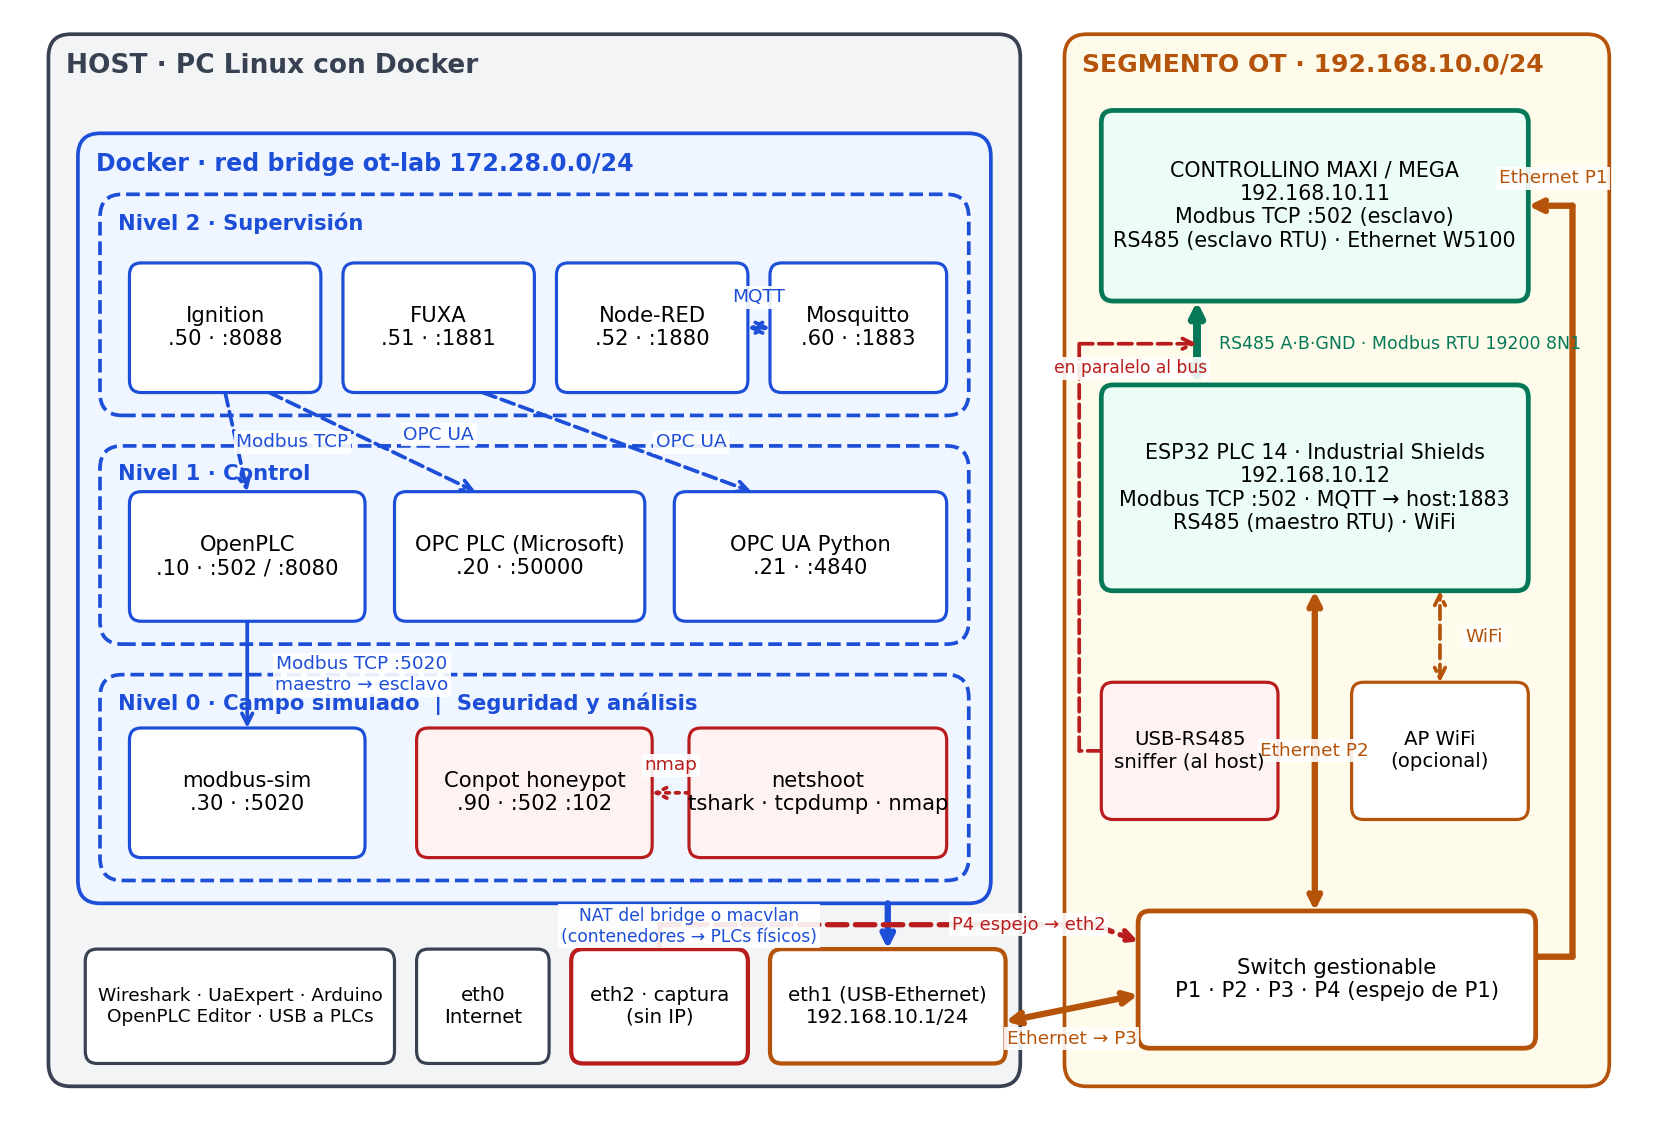
\includegraphics[width=\textwidth]{fig1_topologia}
  \caption{Topología completa del laboratorio: contenedores Docker en el host y segmento OT físico con Controllino y ESP32 PLC~14.}
  \label{fig:topologia}
\end{figure}

\begin{figure}[H]
  \centering
  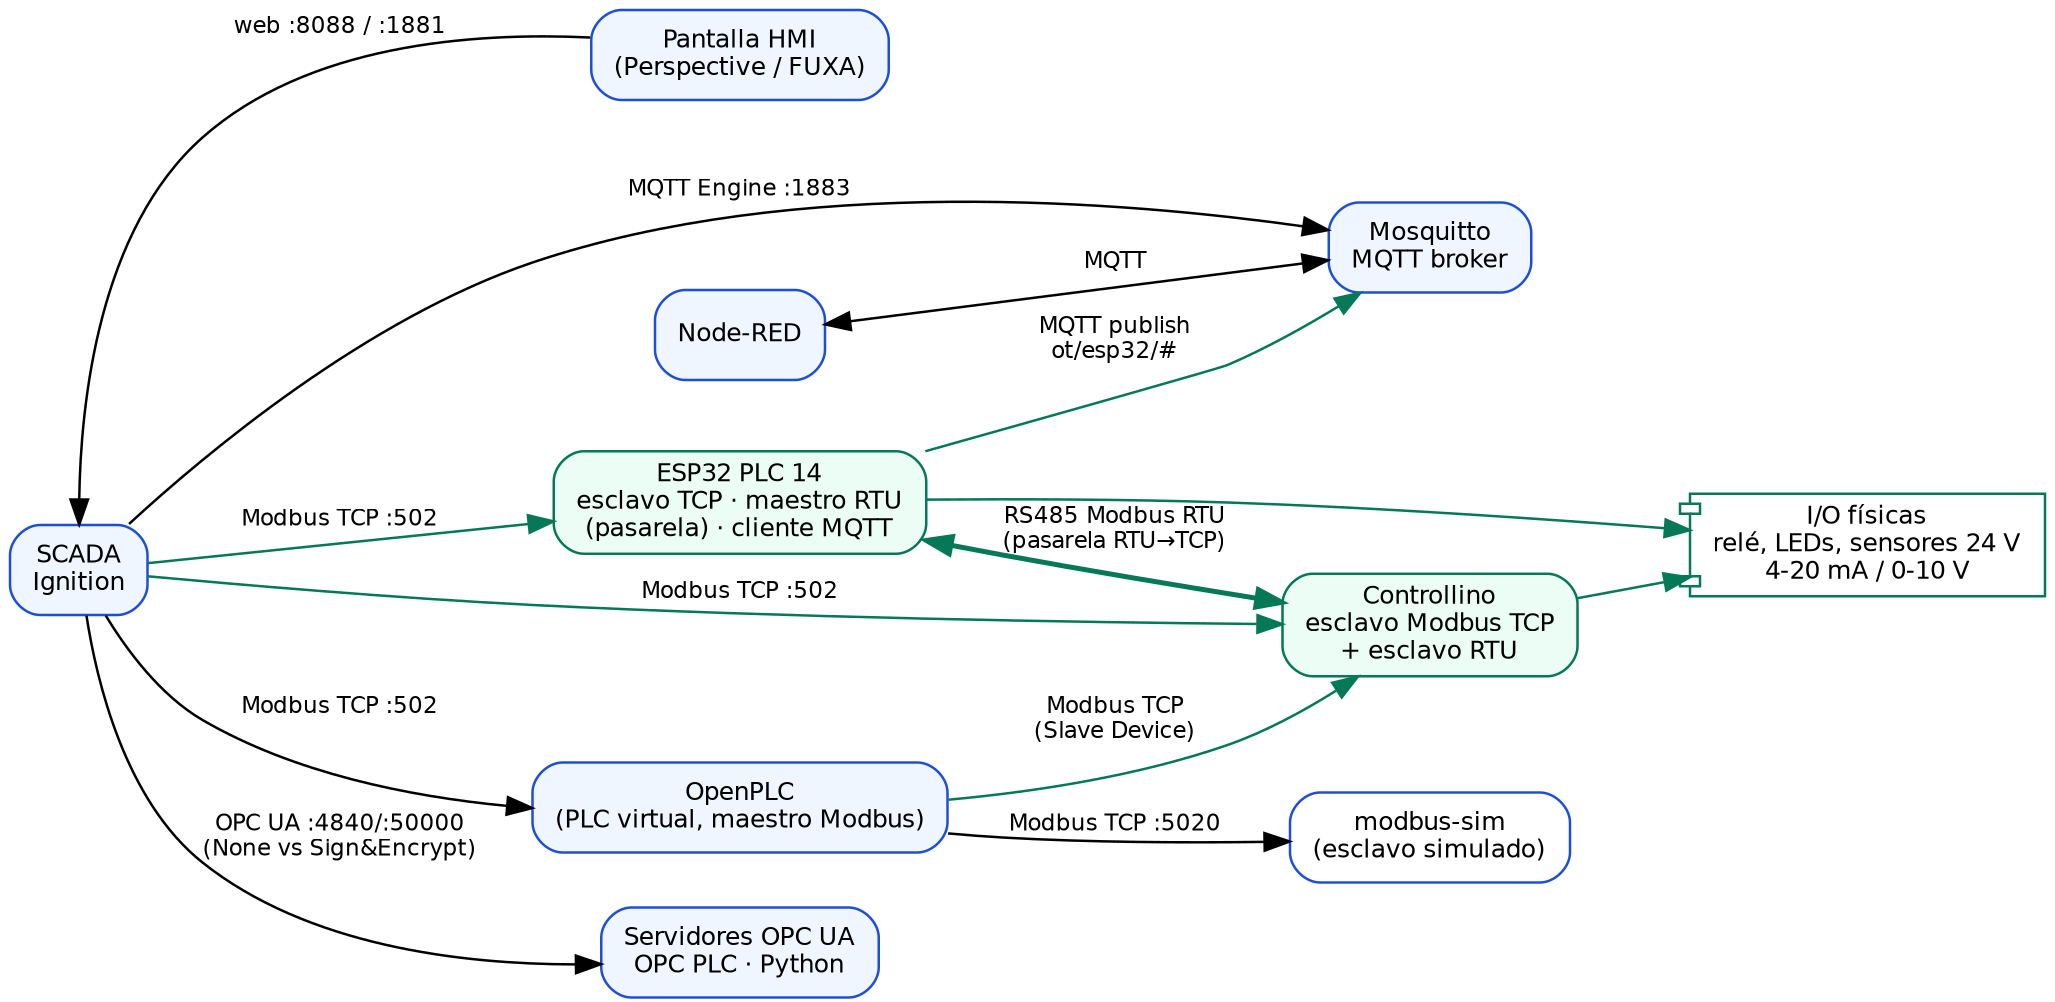
\includegraphics[width=\textwidth]{fig3_flujo}
  \caption{Flujo de datos y protocolos entre los componentes del laboratorio.}
  \label{fig:flujo}
\end{figure}

% -----------------------------------------------------------------------------
\section{Práctica 1 --- Modbus TCP}
\label{sec:prac-modbus}

\subsection{Esclavo simulado: \cmd{modbus-sim}}

El servicio \cmd{modbus-sim} ejecuta \cmd{oitc/modbus-server}, un esclavo Modbus TCP en Python cuyos registros iniciales se definen en \cmd{modbus/server.json} (anexo~\ref{sec:anexo-modbus}). Escucha en el puerto 5020 con estos valores:

\begin{table}[H]
\centering\small
\caption{Registros iniciales del esclavo simulado.}
\begin{tabular}{llll}
\toprule
\textbf{Tabla} & \textbf{Offset} & \textbf{Valor} & \textbf{Notación 1-based} \\
\midrule
Holding registers & 0, 1, 2 & 1234, 25, 72 & 40001--40003 \\
Input registers & 0 & 999 & 30001 \\
Coils & 0, 1 & 0, 1 & 00001--00002 \\
Discrete inputs & 0, 1 & 1, 0 & 10001--10002 \\
\bottomrule
\end{tabular}
\end{table}

\begin{lstlisting}[style=bash]
docker compose up -d modbus-sim
docker compose logs modbus-sim      # "Start Modbus TCP server on 0.0.0.0:5020"
\end{lstlisting}

\subsection{Cliente Modbus desde un contenedor}

Sin instalar nada en el host, un contenedor Python unido a la red \lab{} lee y escribe registros:

\begin{lstlisting}[style=bash]
docker run --rm --network ot-lab python:3.12-slim sh -c \
  "pip -q install pymodbus && python - <<'EOF'
from pymodbus.client import ModbusTcpClient
c = ModbusTcpClient('172.28.0.30', port=5020); c.connect()
print(c.read_holding_registers(0, count=3, slave=1).registers)
c.write_register(1, 42, slave=1)
print(c.read_holding_registers(0, count=3, slave=1).registers)
c.close()
EOF"
\end{lstlisting}

\begin{ok}
Primera línea \cmd{[1234, 25, 72]}; segunda \cmd{[1234, 42, 72]}. La escritura (FC~06) modificó el offset~1.
\end{ok}

Alternativa con \cmd{mbpoll}: \cmd{docker run --rm --network ot-lab debian:bookworm sh -c "apt-get -qq update \&\& apt-get -qq install -y mbpoll >/dev/null \&\& mbpoll -m tcp -a 1 -r 1 -c 3 -p 5020 172.28.0.30 -1"}. Obsérvese que \cmd{mbpoll} usa direcciones 1-based (\cmd{-r 1} es el offset~0).

\subsection{PLC virtual: OpenPLC}
\label{sec:prac-openplc}

\begin{enumerate}
  \item Abrir \url{http://localhost:8080} (\cmd{openplc}/\cmd{openplc}).
  \item \menu{Programs \ra{} Upload}: subir un programa \cmd{.st} (el repositorio de OpenPLC incluye ejemplos; el más simple copia una entrada a una salida) y \menu{Launch program}. \menu{Start PLC}.
  \item \menu{Settings}: comprobar que \emph{Modbus Server} está habilitado en el puerto 502. OpenPLC ya es un esclavo Modbus: sus \cmd{\%QX0.0} son coils 0--7, sus \cmd{\%IW100} registros de entrada, etc.
  \item Para que además actúe como \textbf{maestro} y lea el simulador: \menu{Slave Devices \ra{} Add new device}, protocolo \emph{Generic Modbus TCP Device}, IP \ip{172.28.0.30}, puerto 5020, \emph{Holding Registers -- Read} start 0 size 3. OpenPLC mapea esos registros a \cmd{\%IW100..\%IW102} y los sondea cada 100~ms: ya hay tráfico Modbus continuo entre dos contenedores.
\end{enumerate}

\begin{nota}
OpenPLC, como maestro, abre una conexión TCP al simulador y la mantiene, enviando peticiones FC~03 periódicas. Esa es la primera ``firma'' de sondeo que se analizará en la práctica~\ref{sec:prac-captura}.
\end{nota}

% -----------------------------------------------------------------------------
\section{Práctica 2 --- OPC UA}
\label{sec:prac-opcua}

\subsection{Servidor simulado: OPC PLC}

\cmd{opc-plc} arranca con opciones que generan nodos lentos (\cmd{--sn=5 --sr=10}: 5 nodos cada 10~s), rápidos (\cmd{--fn=5 --fr=1}) y con anomalías (\cmd{--gn=5}), acepta cualquier certificado de cliente (\cmd{--autoaccept}) y permite usuarios anónimos (\cmd{--ut}). Endpoint: \nolinkurl{opc.tcp://localhost:50000} desde el host; \nolinkurl{opc.tcp://172.28.0.20:50000} desde otros contenedores.

\subsection{Servidor propio en Python}

\cmd{opcua-py} se construye desde \cmd{opcua/Dockerfile} y ejecuta \cmd{server.py} (anexo~\ref{sec:anexo-opcua}), que publica el objeto \cmd{Tanque1} con \cmd{Nivel} (senoide 20--80), \cmd{Temperatura} (15--25) y \cmd{Valvula} (booleano escribible). Endpoint: \nolinkurl{opc.tcp://localhost:4840/lab/}. Para modificarlo: editar \cmd{server.py} y \cmd{docker compose up -d --build opcua-py}.

\subsection{Cliente UaExpert}

\begin{enumerate}
  \item \menu{Add Server \ra{} Custom Discovery}: introducir \nolinkurl{opc.tcp://localhost:50000} y \nolinkurl{opc.tcp://localhost:4840/lab/}. UaExpert lista los endpoints de cada servidor con sus políticas.
  \item Conectar primero con \textbf{None / None} (sin seguridad) y anónimo. Navegar hasta \cmd{Objects \ra{} Tanque1 \ra{} Nivel}, arrastrarlo a \emph{Data Access View} y ver cómo cambia cada segundo. Escribir \cmd{true} en \cmd{Valvula}.
  \item Mientras, capturar el tráfico (práctica~\ref{sec:prac-captura}) y observar en Wireshark, con filtro \cmd{opcua}, los mensajes \cmd{Hello}, \cmd{OpenSecureChannel}, \cmd{CreateSession}, \cmd{ActivateSession}, \cmd{Browse}, \cmd{Read}, \cmd{CreateSubscription} y los \cmd{Publish} periódicos, con los valores legibles.
  \item Desconectar y reconectar con \textbf{Basic256Sha256 / Sign \& Encrypt}. Aceptar el certificado del servidor (\emph{Trust Server Certificate}). Repetir la captura: tras el \cmd{OpenSecureChannel} solo se ven mensajes \cmd{MSG} con carga cifrada.
\end{enumerate}

\begin{ok}
Dos capturas: una con valores de \cmd{Nivel} legibles en los \cmd{Publish}, otra donde solo los mensajes \cmd{HEL/ACK}, \cmd{OPN} y los certificados son visibles. Anotar qué campos siguen en claro en la segunda (URL del endpoint, política, certificados X.509).
\end{ok}

Cliente en contenedor, como alternativa a UaExpert:

\begin{lstlisting}[style=bash]
docker run --rm --network ot-lab python:3.12-slim sh -c \
  "pip -q install asyncua && python - <<'EOF'
import asyncio
from asyncua import Client
async def main():
    async with Client('opc.tcp://172.28.0.21:4840/lab/') as c:
        n = await c.nodes.root.get_child(['0:Objects','2:Tanque1','2:Nivel'])
        print('Nivel =', await n.read_value())
asyncio.run(main())
EOF"
\end{lstlisting}

% -----------------------------------------------------------------------------
\section{Práctica 3 --- SCADA}
\label{sec:prac-scada}

\subsection{Ignition}
\label{sec:prac-ignition}

Ignition corre \emph{dentro} de Docker, por lo que debe usar las IPs de la red \lab{}, nunca \cmd{localhost}.

\begin{enumerate}
  \item Entrar en \url{http://localhost:8088} (\cmd{admin}/\cmd{lab1234!}); rechazar el Quick Start (sección~\ref{sec:ignition-primer}).
  \item \menu{Config \ra{} OPC UA \ra{} Device Connections \ra{} Create new Device \ra{} Modbus TCP}: nombre \cmd{OpenPLC}, host \ip{172.28.0.10}, puerto 502. Repetir con nombre \cmd{ModbusSim}, host \ip{172.28.0.30}, puerto 5020. En cada dispositivo, pestaña \emph{Advanced}: \emph{Max concurrent requests}~=~1 si se va a comparar con los PLC físicos.
  \item En el dispositivo Modbus, \menu{More \ra{} Addresses}: definir un rango, p.\,ej. prefijo \cmd{HR}, tipo \emph{HoldingRegister}, inicio 1, fin 3 (Ignition usa direcciones 1-based). Esto genera tags navegables.
  \item \menu{Config \ra{} OPC UA \ra{} Connections \ra{} Create new}: endpoint \nolinkurl{opc.tcp://172.28.0.20:50000} y otro \nolinkurl{opc.tcp://172.28.0.21:4840/lab/}, política \cmd{None} para empezar. Ignition también expone su propio servidor OPC UA en el 62541.
  \item \menu{Status \ra{} Connections \ra{} Devices} debe mostrar los dispositivos como \emph{Connected}.
  \item Descargar el \textbf{Designer Launcher} desde la página principal del Gateway, añadir el Gateway \cmd{localhost:8088}, abrir el Designer, crear un proyecto Perspective, arrastrar desde el \emph{Tag Browser} (\cmd{[default]} \ra{} dispositivos) los tags \cmd{HR1..HR3} y \cmd{Tanque1/Nivel} a una vista y guardar. Abrir la sesión Perspective en el navegador.
\end{enumerate}

\begin{ok}
Los valores del simulador (1234, 25, 72) y el \cmd{Nivel} senoidal aparecen en la vista Perspective y se actualizan. Al capturar en \cmd{ignition} se ve un sondeo Modbus regular (por defecto cada 1~s, tag group \emph{Default}) hacia cada dispositivo y un \cmd{Publish} OPC UA hacia cada servidor.
\end{ok}

\subsection{FUXA}

En \url{http://localhost:1881}: \menu{Connections \ra{} +}: tipo \emph{ModbusTCP}, IP \ip{172.28.0.30}, puerto 5020, esclavo~1; añadir tags con dirección 40001--40003 (FUXA usa notación 1-based con prefijo). Otra conexión \emph{OPC UA} a \nolinkurl{opc.tcp://172.28.0.21:4840/lab/} y navegar hasta \cmd{Tanque1}. Crear una vista con un \emph{gauge} enlazado a \cmd{Nivel}. Comparar en Wireshark el patrón de sondeo de FUXA con el de Ignition: número de conexiones TCP y periodo.

\subsection{Node-RED}

En \url{http://localhost:1880}: \menu{Manage palette \ra{} Install}: \cmd{node-red-contrib-modbus} y \cmd{node-red-contrib-opcua}. Flujo mínimo: nodo \emph{Modbus Read} (servidor \ip{172.28.0.30}:5020, FC~3, dirección 0, cantidad 3, cada 500~ms) \ra{} \emph{debug}. Segundo flujo: \emph{OpcUa Client} suscrito a \cmd{ns=2;s=...} \ra{} \emph{mqtt out} hacia \ip{172.28.0.60} topic \cmd{ot/nodered/nivel}. Node-RED se convierte así en pasarela OPC UA\ra{}MQTT y en generador de tráfico continuo.

% -----------------------------------------------------------------------------
\section{Práctica 4 --- Captura y análisis de tráfico}
\label{sec:prac-captura}

\subsection{Capturar dentro de la red Docker con netshoot}

El método universal (Linux, macOS, Windows) es unir un contenedor \cmd{netshoot} al namespace de red del servicio a observar:

\begin{lstlisting}[style=bash]
# Ver 30 s de trafico Modbus que llega a OpenPLC, decodificado
docker run --rm --net container:openplc nicolaka/netshoot \
  tshark -i eth0 -a duration:30 -f "tcp port 502" -Y modbus

# Guardar a pcap el trafico OPC UA del servidor Microsoft, para abrirlo en Wireshark
docker run --rm --net container:opc-plc -v "$PWD/captures:/cap" nicolaka/netshoot \
  tcpdump -i eth0 -w /cap/opcua.pcap "tcp port 50000"

# Todo lo que entra y sale de Ignition (sondeo a todos los dispositivos)
docker run --rm --net container:ignition -v "$PWD/captures:/cap" nicolaka/netshoot \
  tcpdump -i eth0 -w /cap/ignition.pcap "not port 8088"
\end{lstlisting}

Los archivos aparecen en \cmd{captures/} del host y se abren con Wireshark. Ctrl+C detiene la captura.

\subsection{Capturar desde el host (solo Linux)}

\begin{lstlisting}[style=bash]
docker network inspect ot-lab -f '{{.Id}}' | cut -c1-12      # -> br-<id>
sudo wireshark -i br-<id> -k -f "tcp port 502 or tcp port 5020 or tcp port 50000 or tcp port 4840"
\end{lstlisting}

\subsection{Filtros útiles en Wireshark}

\begin{table}[H]
\centering\small
\caption{Filtros de visualización de Wireshark para el laboratorio.}
\label{tab:filtros}
\begin{tabularx}{\textwidth}{L{5.6cm} X}
\toprule
\textbf{Filtro} & \textbf{Qué muestra} \\
\midrule
\cmd{mbtcp} & Modbus TCP completo (MBAP + PDU) \\
\cmd{modbus.func\_code == 3} & Lecturas de holding registers \\
\cmd{modbus.func\_code in \{5 6 15 16\}} & Todas las escrituras (coils y registros) \\
\cmd{modbus.exception\_code} & Respuestas de excepción \\
\cmd{opcua} & OPC UA (decodifica en claro solo con None/None) \\
\cmd{opcua.transport.type == "HEL"} & Inicio de conexiones OPC UA \\
\cmd{opcua.servicenodeid.numeric == 631} & Publish requests \\
\cmd{mqtt} & MQTT; \cmd{mqtt.msgtype == 3} solo PUBLISH \\
\cmd{s7comm} & Tráfico S7 (contra Conpot) \\
\cmd{tcp.analysis.retransmission} & Retransmisiones (ejercicio WiFi) \\
\cmd{ip.addr == 172.28.0.50} & Todo lo que toca a Ignition \\
\bottomrule
\end{tabularx}
\end{table}

\menu{Statistics \ra{} Conversations} resume quién habla con quién; \menu{Statistics \ra{} I/O Graph} con el filtro \cmd{mbtcp} muestra el sondeo como una señal periódica: un SCADA leyendo cada segundo es una firma que conviene reconocer a simple vista. Si OPC UA en el 50000 no se decodifica: \menu{Analyze \ra{} Decode As \ra{} TCP port 50000 \ra{} OpcUa}.

\subsection{Reconocimiento con nmap}

\begin{lstlisting}[style=bash]
# Inventario de la red del laboratorio
docker run --rm --network ot-lab nicolaka/netshoot \
  nmap -sT -p 502,5020,102,4840,50000,8080,1881,8088,1883 172.28.0.0/24

# Scripts NSE especificos de ICS
docker run --rm --network ot-lab nicolaka/netshoot \
  nmap -p 502 --script modbus-discover 172.28.0.10 172.28.0.30
\end{lstlisting}

\begin{ok}
nmap identifica nueve hosts activos y sus puertos; \cmd{modbus-discover} devuelve el \emph{slave ID} y, en OpenPLC, el identificador del dispositivo. A partir solo de puertos y banners debe poder clasificarse cada host por función (ejercicio~4 del capítulo~\ref{cap:ejercicios}).
\end{ok}

% -----------------------------------------------------------------------------
\section{Práctica 5 --- Honeypot ICS con Conpot}
\label{sec:prac-conpot}

Conpot simula un Siemens S7-300 (S7comm en el 102, Modbus en el 502, SNMP en el 161 y web en el 80). Sus puertos están publicados en el host con prefijo 10 (10102, 10502, 10080, 10161) para no chocar con OpenPLC.

\begin{lstlisting}[style=bash]
docker run --rm --network ot-lab nicolaka/netshoot \
  nmap -p 502,102 --script modbus-discover,s7-info 172.28.0.90
docker compose logs -f conpot
\end{lstlisting}

\begin{ok}
\cmd{s7-info} devuelve modelo, número de serie y versión de firmware ``del PLC''; el log de Conpot registra cada conexión con IP de origen, protocolo y función solicitada, exactamente como lo haría un IDS. Abrir \url{http://localhost:10080} muestra la web de diagnóstico falsa.
\end{ok}

Escribir después un registro Modbus en Conpot desde pymodbus (\ip{172.28.0.90}, puerto 502) y correlacionar la entrada del log con la captura: es el ejercicio~6.

\chapter{Práctica 6 --- Integración de los PLC físicos}
\label{cap:hardware}

Aquí el laboratorio deja de ser simulado. El Controllino y el ESP32 PLC~14 se programan con Arduino IDE (o con OpenPLC Editor) y hablan Modbus, así que encajan como dispositivos de nivel~1/0 que Ignition, FUXA y el OpenPLC de Docker pueden leer y escribir.

\section{Equipos}

\begin{table}[H]
\centering\small
\caption{Características de los dos PLC físicos y su papel en el laboratorio.}
\label{tab:plcs}
\begin{tabularx}{\textwidth}{L{2.4cm} X X}
\toprule
 & \textbf{Controllino} & \textbf{ESP32 PLC 14 (Industrial Shields)} \\
\midrule
MCU & ATmega2560 (MAXI/MEGA) o ATmega328 (MINI), 16~MHz & ESP32 doble núcleo 240~MHz \\
Ethernet & Sí en MAXI/MEGA (W5100, 10/100). \textbf{MINI no tiene} & Sí (RJ45) \\
Inalámbrico & No & WiFi + BLE \\
Serie industrial & RS485 en MAXI/MEGA & RS485 half-duplex \\
Otros & RTC, E/S 24~V, relés & I2C de expansión, RTC, E/S 24~V, 1 relé, entradas 0--10~V / 4--20~mA \\
Rol en el lab & Esclavo Modbus TCP ``clásico'', cableado, lento y determinista & Esclavo Modbus TCP, pasarela RTU\ra{}TCP, publicador MQTT; comparar Ethernet frente a WiFi \\
\bottomrule
\end{tabularx}
\end{table}

\begin{nota}
Si el Controllino es \textbf{MINI} (sin Ethernet ni RS485), conectarlo por USB y usarlo como esclavo Modbus RTU sobre serie; el host o el ESP32 hacen de pasarela. El resto del capítulo asume MAXI o MEGA.
\end{nota}

\section{Topología física y direccionamiento}

\begin{figure}[H]
  \centering
  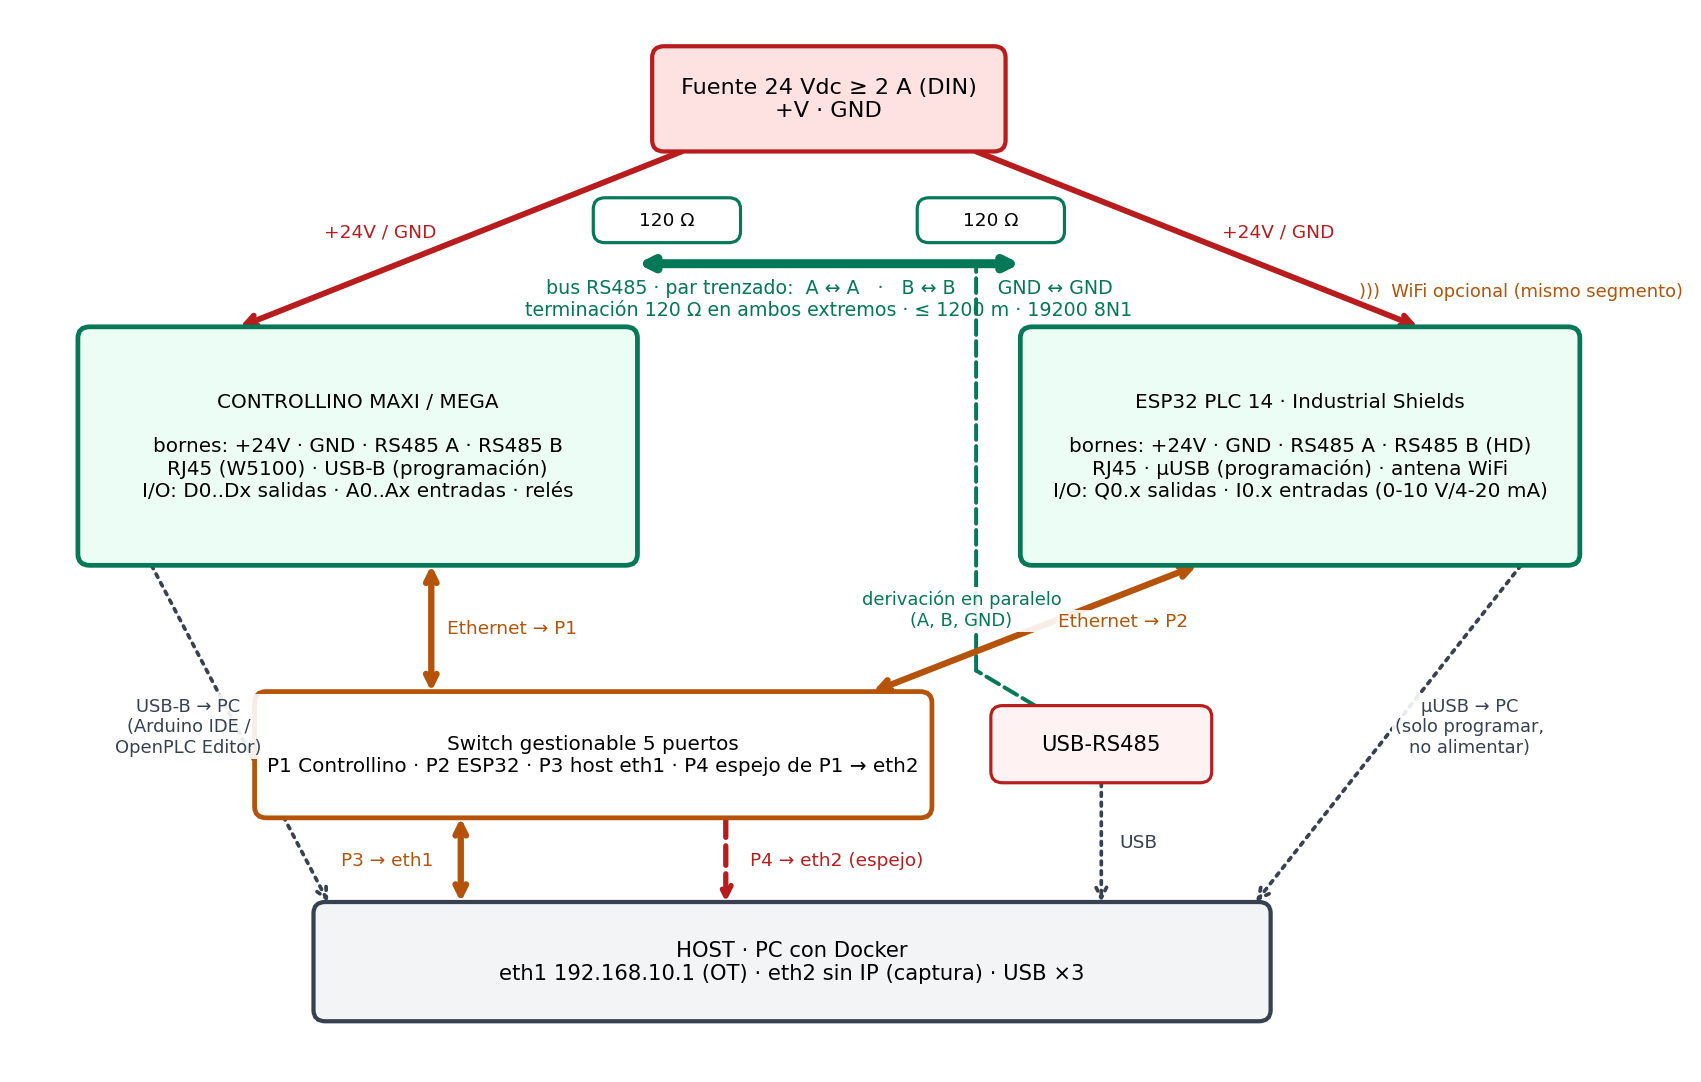
\includegraphics[width=\textwidth]{fig4_cableado}
  \caption{Conexiones físicas: alimentación, Ethernet, bus RS485 y USB de programación.}
  \label{fig:cableado}
\end{figure}

\begin{enumerate}
  \item Conectar la segunda NIC del host (\cmd{eth1}, USB-Ethernet), el Controllino y el ESP32 a un switch. Alimentar ambos PLC a 24~V desde la fuente, no por USB.
  \item IPs estáticas: host \ip{192.168.10.1/24}, Controllino \ip{.11}, ESP32 \ip{.12}. Sin puerta de enlace en los PLC: no tienen por qué salir a ningún sitio.
  \item Configurar la NIC del host y comprobar conectividad:
\begin{lstlisting}[style=bash]
# Linux
sudo ip addr add 192.168.10.1/24 dev eth1 && sudo ip link set eth1 up
# macOS: Ajustes -> Red -> adaptador USB -> Configurar IPv4: Manual, 192.168.10.1 / 255.255.255.0
ping -c 3 192.168.10.11 && ping -c 3 192.168.10.12
\end{lstlisting}
  \item Si el switch es gestionable, configurar \emph{port mirroring} del puerto del Controllino hacia un puerto donde haya una tercera NIC de captura (\cmd{eth2}, sin IP). Wireshark verá el tráfico SCADA $\leftrightarrow$ PLC aunque no pase por el host: es la posición de un sensor pasivo de red OT.
\end{enumerate}

El segmento \ip{192.168.10.0/24} va en una NIC dedicada, separado de la red doméstica o de la universidad: eso ya es un ejercicio de segmentación.

\section{Cómo llegan los contenedores a los PLC}
\label{sec:nat-macvlan}

\textbf{A) Bridge + NAT (por defecto; cualquier SO).} Los contenedores salen por NAT del host, así que Ignition, FUXA y OpenPLC alcanzan \ip{192.168.10.11:502} sin configurar nada. Limitación: los PLC no pueden iniciar conexiones hacia un contenedor salvo a través de un puerto publicado en el host (el ESP32 publica MQTT a \ip{192.168.10.1:1883}, que es el puerto publicado de Mosquitto). En Wireshark, todo el tráfico de los contenedores aparece con la IP del host.

\textbf{B) macvlan (solo Linux nativo).} Cada contenedor recibe una IP y una MAC propias en \ip{192.168.10.0/24}; en Wireshark aparecen como equipos distintos y se puede hacer nmap ``desde fuera''.

\begin{lstlisting}[style=yaml]
networks:
  ot-phys:
    driver: macvlan
    driver_opts:
      parent: eth1
    ipam:
      config:
        - subnet: 192.168.10.0/24
          ip_range: 192.168.10.128/25   # rango reservado a contenedores
          gateway: 192.168.10.1
\end{lstlisting}

Añadir a \cmd{ignition}, \cmd{fuxa}, \cmd{node-red} y \cmd{openplc} una segunda red \cmd{ot-phys: \{ ipv4\_address: 192.168.10.150 \}} (y sucesivas). Con macvlan el host \emph{no} puede hablar con sus propios contenedores por \cmd{eth1}; hace falta una interfaz puente:

\begin{lstlisting}[style=bash]
sudo ip link add ot-shim link eth1 type macvlan mode bridge
sudo ip addr add 192.168.10.2/32 dev ot-shim && sudo ip link set ot-shim up
sudo ip route add 192.168.10.128/25 dev ot-shim
\end{lstlisting}

\section{Firmware: opción rápida con OpenPLC Editor}

OpenPLC Editor compila un programa IEC 61131-3 y lo sube directamente a placas Arduino, incluidos Controllino MAXI/MEGA/MINI y ESP32, dejando la placa como esclavo Modbus (TCP y/o RTU) con las E/S mapeadas a \cmd{\%IX}, \cmd{\%QX}, \cmd{\%IW}, \cmd{\%QW}.

\begin{enumerate}
  \item Nuevo proyecto; escribir un ladder sencillo (p.\,ej. \cmd{\%QX0.0 := \%IX0.0}).
  \item \menu{Transfer program to PLC}: \emph{Board} = Controllino MAXI o ESP32; pestaña \menu{Modbus}: habilitar TCP, IP \ip{192.168.10.11} (Controllino) o \ip{.12} (ESP32), puerto 502; en el ESP32 elegir Ethernet o WiFi (SSID/clave).
  \item Compilar y subir. El dispositivo ya responde Modbus TCP.
  \item En el OpenPLC de Docker (\url{http://localhost:8080}) \menu{Slave Devices \ra{} Add}: Generic Modbus TCP, IP del PLC físico, mapear sus registros. El PLC virtual controla ahora E/S reales. En Ignition, añadir ambos como dispositivos Modbus TCP igual que el simulador.
\end{enumerate}

Industrial Shields documenta el mapa de pines de sus placas; comprobar qué pines Arduino corresponden a I0.x/Q0.x antes de usarlos desde OpenPLC.

\section{Firmware: opción con Arduino IDE (control total)}

Instalar en Arduino IDE el paquete de placas \cmd{industrialshields-esp32} y la librería \textbf{Tools40} (clases \cmd{ModbusTCPSlave}, \cmd{ModbusTCPMaster}, \cmd{ModbusRTUSlave}, \cmd{ModbusRTUMaster}); para el Controllino, las placas Controllino y la librería \textbf{ArduinoModbus} (con ArduinoRS485).

\textbf{ESP32 PLC 14 como esclavo Modbus TCP por Ethernet} (esqueleto; partir de \menu{File \ra{} Examples \ra{} Tools40} para el modelo exacto):

\begin{lstlisting}[style=cpp]
#include <Ethernet.h>
#include <ModbusTCPSlave.h>

byte mac[] = {0xDE,0xAD,0xBE,0xEF,0x00,0x12};
IPAddress ip(192,168,10,12);
ModbusTCPSlave modbus(502);

bool     coils[4];
bool     dinputs[4];
uint16_t hregs[4];
uint16_t iregs[4];

void setup() {
  Ethernet.begin(mac, ip);
  modbus.begin();
  modbus.setCoils(coils, 4);
  modbus.setDiscreteInputs(dinputs, 4);
  modbus.setHoldingRegisters(hregs, 4);
  modbus.setInputRegisters(iregs, 4);
}

void loop() {
  dinputs[0] = digitalRead(I0_0);
  iregs[0]   = analogRead(I0_5);      // entrada analogica
  digitalWrite(Q0_0, coils[0]);      // el SCADA escribe el coil 0 -> sale por Q0.0
  modbus.update();
}
\end{lstlisting}

\textbf{Controllino MAXI como esclavo Modbus TCP} (ArduinoModbus):

\begin{lstlisting}[style=cpp]
#include <Controllino.h>
#include <SPI.h>
#include <Ethernet.h>
#include <ArduinoRS485.h>
#include <ArduinoModbus.h>

byte mac[] = {0xDE,0xAD,0xBE,0xEF,0x00,0x11};
EthernetServer server(502);
ModbusTCPServer modbusTCP;

void setup() {
  Ethernet.begin(mac, IPAddress(192,168,10,11));
  server.begin();
  modbusTCP.begin();
  modbusTCP.configureCoils(0, 8);
  modbusTCP.configureDiscreteInputs(0, 8);
  modbusTCP.configureHoldingRegisters(0, 8);
  pinMode(CONTROLLINO_D0, OUTPUT);
  pinMode(CONTROLLINO_A0, INPUT);
}

void loop() {
  EthernetClient client = server.available();
  if (client) {
    modbusTCP.accept(client);
    while (client.connected()) {
      modbusTCP.poll();
      modbusTCP.discreteInputWrite(0, digitalRead(CONTROLLINO_A0));
      digitalWrite(CONTROLLINO_D0, modbusTCP.coilRead(0));
    }
  }
}
\end{lstlisting}

Comprobar desde el host: \cmd{mbpoll -m tcp -a 1 -t 0 -r 1 -c 4 192.168.10.11} (leer coils) y \cmd{mbpoll -m tcp -a 1 -t 0 -r 1 192.168.10.11 1} (escribir el coil~0): debe oírse el relé o verse el LED de salida.

\section{Modbus RTU sobre RS485 entre los dos PLC}
\label{sec:rtu}

Cablear A $\leftrightarrow$ A, B $\leftrightarrow$ B y GND entre el RS485 del Controllino y el del ESP32, con terminación de 120~$\Omega$ en ambos extremos. Controllino como \textbf{esclavo RTU} (\cmd{ModbusRTUServer} de ArduinoModbus, 19200~8N1, ID~1); ESP32 como \textbf{maestro RTU} (\cmd{ModbusRTUMaster} de Tools40) que lee los registros del Controllino y los copia en sus propios \emph{holding registers} Modbus TCP. Desde Ignition se lee el Controllino ``a través'' del ESP32, que actúa de \textbf{pasarela RTU\ra{}TCP}, exactamente lo que hacen los gateways Moxa o Anybus en planta.

Para analizar el bus serie: el adaptador USB-RS485 del host se conecta en paralelo al bus (A, B, GND) y se capturan los bytes crudos con \cmd{pymodbus} (\cmd{ModbusSerialClient}, \cmd{framer='rtu'}) o con un script que vuelque \cmd{serial.read()} en hexadecimal. Wireshark no lee serie directamente; se puede exponer el puerto por TCP con \cmd{socat} y decodificar como \cmd{mbrtu} con \menu{Decode As}.

\section{MQTT desde el ESP32}
\label{sec:mqtt-esp32}

El broker Mosquitto ya está en el compose (\ip{172.28.0.60:1883}, publicado en el host). En el ESP32, con la librería \cmd{PubSubClient}, conectar a \ip{192.168.10.1:1883}, publicar cada segundo \cmd{ot/esp32/nivel} y suscribirse a \cmd{ot/esp32/cmd}. Node-RED (nodo \emph{mqtt in}) e Ignition (módulo MQTT Engine) lo consumen. Ejercicio de red: MQTT viaja en claro sobre TCP 1883; capturar, leer el payload, y después habilitar un listener TLS en el 8883 de Mosquitto (certificado autofirmado, \cmd{cafile}/\cmd{certfile}/\cmd{keyfile} en \cmd{mosquitto.conf} y republicar el puerto) para ver la diferencia. Cambiar el ESP32 de Ethernet a WiFi y comparar el \emph{jitter} en \menu{Statistics \ra{} I/O Graph} con el filtro \cmd{mqtt}.

\chapter{Ejercicios propuestos}
\label{cap:ejercicios}

Los ejercicios están ordenados de menor a mayor dificultad y cada uno se apoya en los anteriores. Para cada uno se espera una captura \cmd{.pcap} comentada, las respuestas a las preguntas y, cuando proceda, la configuración empleada.

\section{Con el laboratorio en Docker}

\begin{enumerate}[label=\textbf{E\arabic*.},leftmargin=*,itemsep=4pt]
  \item \textbf{Anatomía Modbus.} Capturar una lectura (FC~03) y una escritura (FC~06) contra \cmd{modbus-sim}. Identificar en la MBAP el \emph{transaction ID}, el \emph{unit ID} y el campo \emph{length}; en la PDU el código de función, la dirección y los datos. Provocar una excepción leyendo un registro fuera de rango (offset 70000 no es posible; usar el FC~04 sobre \cmd{openplc} en un offset alto) y explicar el código devuelto.
  \item \textbf{Polling.} Configurar en Ignition un \emph{tag group} de 500~ms para el dispositivo OpenPLC y medir en I/O Graph los paquetes por segundo. Cambiar a 100~ms y comparar. ¿Cuántas peticiones genera Ignition por ciclo y por qué? ¿Cómo agrupa registros contiguos?
  \item \textbf{OPC UA en claro frente a cifrado.} Dos capturas de UaExpert (None/None frente a Basic256Sha256 Sign\&Encrypt). Explicar qué sigue siendo visible (endpoints, políticas, certificados, tamaños y periodicidad) y qué deja de serlo. ¿Qué podría inferir un atacante pasivo de la sesión cifrada?
  \item \textbf{Reconocimiento.} Con nmap sobre \ip{172.28.0.0/24} y sin consultar el compose, clasificar cada host por función solo a partir de puertos y banners. Después ejecutar \cmd{modbus-discover} y \cmd{s7-info} y anotar qué información adicional exponen los protocolos ICS sin autenticación.
  \item \textbf{Segmentación.} Crear una segunda red \cmd{ot-dmz} en el compose, mover Ignition a ella y dejar Node-RED conectado a ambas como pasarela. Verificar con nmap desde Ignition que ya no ve a OpenPLC directamente, y montar en Node-RED un flujo que le ``publique'' los datos por OPC UA o MQTT. Discutir qué se gana y qué se pierde.
  \item \textbf{Detección.} Lanzar un escaneo y una escritura Modbus no autorizada contra Conpot. Correlacionar cada línea del log del honeypot con los paquetes de la captura. Proponer una regla de alerta (p.\,ej. Suricata: cualquier FC de escritura hacia el 502 desde una IP distinta del SCADA).
  \item \textbf{Manipulación.} Desde pymodbus escribir un coil de OpenPLC mientras Ignition lo muestra en pantalla. Observar el efecto en la HMI y localizar la escritura en la captura. ¿Cómo distinguiría un operador una escritura legítima del SCADA de una externa, si ambas son idénticas en el cable?
\end{enumerate}

\section{Con los PLC físicos}

\begin{enumerate}[label=\textbf{E\arabic*.},leftmargin=*,itemsep=4pt,resume]
  \item \textbf{Simulado frente a real.} Ignition sondea a la vez \cmd{modbus-sim}, OpenPLC (Docker) y el Controllino. En Wireshark comparar el \emph{delta time} petición\ra{}respuesta de cada uno (columna \cmd{modbus.response\_time} o \cmd{tcp.time\_delta}). El Controllino (W5100, AVR a 16~MHz) será visiblemente más lento. ¿Qué implica para el periodo mínimo de sondeo del SCADA?
  \item \textbf{Port mirroring.} Capturar el tráfico Ignition $\leftrightarrow$ Controllino desde la NIC conectada al puerto espejo del switch, sin tocar el host. Comparar con la captura desde \cmd{eth1}: ¿qué tráfico aparece en una y no en la otra?
  \item \textbf{Ethernet frente a WiFi.} Mismo firmware en el ESP32 por cable y por WiFi; medir latencia, \emph{jitter} y retransmisiones (\cmd{tcp.analysis.retransmission}). Añadir interferencia (microondas, descargas en la misma WiFi) y repetir. Concluir sobre el uso de WiFi en control.
  \item \textbf{Pasarela RTU\ra{}TCP.} Implementar la sección~\ref{sec:rtu} y observar que una sola petición Modbus TCP al ESP32 desencadena tráfico RS485 hacia el Controllino. Medir el tiempo extra que añade la pasarela.
  \item \textbf{Segmentación real.} Con \cmd{nftables} (Linux) en el host permitir solo TCP~502 desde la IP de Ignition hacia \ip{192.168.10.0/24}. Verificar con nmap desde otro contenedor que ya no alcanza los PLC; intentar la escritura de coil desde un equipo de la red doméstica y comprobar que falla.
  \item \textbf{Escritura no autorizada con efecto físico.} Desde un tercer host escribir el coil del relé del Controllino o del ESP32 y verlo conmutar. Diseñar una regla de detección (Zeek o Suricata con reglas Modbus) que alerte de escrituras desde IPs distintas del SCADA y comprobar que dispara.
  \item \textbf{MQTT en claro frente a TLS.} Sección~\ref{sec:mqtt-esp32}: comparar capturas en 1883 y 8883. ¿Qué metadatos siguen visibles con TLS (tamaño, periodicidad, SNI)?
\end{enumerate}

\begin{nota}[Entregable sugerido por ejercicio]
Archivo \cmd{.pcap} (o \cmd{.pcapng}) con un filtro de visualización guardado, una captura de pantalla de Wireshark con los campos relevantes señalados, y un párrafo de conclusiones. Para los ejercicios de configuración, el fragmento de \cmd{docker-compose.yml} o de firmware modificado.
\end{nota}

\chapter{Problemas frecuentes}
\label{cap:problemas}

Los cuatro fallos de la puesta en marcha (Conpot, \cmd{modbus-sim}, Ignition, imágenes \cmd{amd64}) se describen con detalle en la sección~\ref{sec:fallos}. Esta lista recoge el resto de situaciones habituales.

\begin{longtable}{L{4.6cm} L{10.8cm}}
\caption{Problemas frecuentes y solución.}\label{tab:problemas}\\
\toprule
\textbf{Síntoma} & \textbf{Causa y solución} \\
\midrule
\endfirsthead
\toprule
\textbf{Síntoma} & \textbf{Causa y solución} \\
\midrule
\endhead
\bottomrule
\endfoot
Un contenedor queda en \emph{Restarting} & Ver su log: \cmd{docker compose logs --tail 40 <servicio>}. Casi siempre es un archivo de configuración montado con formato incorrecto o un cambio de esquema tras \cmd{pull}. Fijar la etiqueta de versión de la imagen. \\
Puerto 502 ocupado o requiere privilegios & En Linux, mapear \cmd{"1502:502"} si no se quiere correr Docker como root o algo ya escucha en 502. En macOS Docker Desktop publica puertos bajos sin problema. \\
\cmd{exec format error} & Imagen \cmd{amd64} en host ARM. Añadir \cmd{platform: linux/amd64} o construir la imagen localmente. \\
Ignition muy lento en Apple Silicon & La imagen de Ignition es multi-arquitectura y corre nativa; la lentitud viene de memoria escasa. Asignar $\geq$6~GB a Docker Desktop. OpenPLC y Conpot sí van emulados: activar Rosetta. \\
UaExpert no conecta a \cmd{opc-plc} & El certificado del servidor debe estar en \emph{Trusted} en UaExpert; con \cmd{--autoaccept} el servidor acepta el del cliente, pero el cliente debe aceptar el del servidor. \\
Ignition no ve los contenedores & Usar las IPs de la red \lab{} (\ip{172.28.0.x}), no \cmd{localhost}: Ignition corre dentro de Docker. \\
Ignition no ve los PLC físicos & En modo NAT (opción A) debe alcanzarlos por la IP real (\ip{192.168.10.x}); comprobar con \cmd{docker run --rm --network ot-lab nicolaka/netshoot ping 192.168.10.11}. \\
Módulos de Ignition detenidos, HMI congelada & Ha expirado el trial de 2~h. Pulsar \menu{Reset Trial} en la cabecera del Gateway. \\
Wireshark no decodifica OPC UA & \menu{Analyze \ra{} Decode As \ra{} TCP port 4840/50000 \ra{} OpcUa}. \\
Wireshark no muestra la interfaz \cmd{br-xxxx} & Solo existe en Linux nativo. En macOS/Windows capturar con netshoot dentro de la red Docker. \\
\cmd{netshoot} no captura nada & Verificar que el nombre en \cmd{--net container:<nombre>} coincide con \cmd{container\_name} y que hay tráfico (un sondeo activo desde Ignition u OpenPLC). \\
El Controllino responde a ping pero no a Modbus & El W5100 admite solo 4 sockets simultáneos; cerrar clientes (mbpoll, Ignition, FUXA cuentan). Ignition abre varias conexiones por dispositivo: limitar a 1 en la configuración del dispositivo. \\
El ESP32 se reinicia al recibir tráfico & Alimentación insuficiente por USB. Alimentarlo a 24~V. \\
macvlan no funciona & Solo en Linux nativo con NIC física cableada (no en Docker Desktop, no sobre WiFi, que suele filtrar MAC ajenas). Usar la opción A (NAT). \\
RS485 con datos corruptos & Revisar polaridad A/B, GND común y activar la terminación de 120~$\Omega$ en ambos extremos (el ESP32 PLC~14 y el Controllino tienen jumper o interruptor para ello). \\
Node-RED sin permisos sobre \cmd{nodered-data} (Linux) & El contenedor corre como uid 1000. \cmd{sudo chown -R 1000:1000 nodered-data}. \\
\cmd{docker compose pull} rompe algo que funcionaba & Una imagen \cmd{latest} cambió. Volver a la versión anterior fijando la etiqueta o restaurar \cmd{docker-compose.linux.yml.bak}. \\
\end{longtable}


\appendix
\chapter{Archivos de configuración}
\label{cap:anexos}

Los archivos siguientes se incluyen desde la carpeta \cmd{src/} de esta guía y son copia exacta de los que hay en \lab{}.

\section{\cmd{docker-compose.yml} (versión macOS / Docker Desktop)}
\label{sec:anexo-compose}
\lstinputlisting[style=yaml]{src/docker-compose.yml}

\section{\cmd{docker-compose.windows.yml} (Windows / WSL 2)}
\label{sec:anexo-compose-win}
Volúmenes con nombre para Ignition, FUXA y Node-RED; ver sección~\ref{sec:windows}.
\lstinputlisting[style=yaml]{src/docker-compose.windows.yml}

\section{\cmd{docker-compose.yml} (versión original Linux)}
\label{sec:anexo-compose-linux}
Diferencias respecto a la versión macOS: sin \cmd{platform}, sin \cmd{restart}, Ignition con bind mount y Conpot con \cmd{command} corto; en Linux nativo estas dos últimas también fallan (sección~\ref{sec:fallos}), por lo que se recomienda usar la versión macOS en todos los sistemas.
\lstinputlisting[style=yaml]{src/docker-compose.linux.yml}

\section{\cmd{modbus/server.json}}
\label{sec:anexo-modbus}
\lstinputlisting[style=json]{src/server.json}

\section{\cmd{opcua/server.py} y \cmd{opcua/Dockerfile}}
\label{sec:anexo-opcua}
\lstinputlisting[style=python]{src/server.py}
\lstinputlisting[style=docker]{src/Dockerfile}

\section{\cmd{mosquitto/mosquitto.conf}}
\label{sec:anexo-mosquitto}
\lstinputlisting[style=plain]{src/mosquitto.conf}

Para el ejercicio TLS, añadir un segundo listener con certificados generados con OpenSSL (o \cmd{mkcert}) y publicar el 8883 en el compose:

\begin{lstlisting}[style=plain]
listener 1883
allow_anonymous true

listener 8883
cafile   /mosquitto/certs/ca.crt
certfile /mosquitto/certs/server.crt
keyfile  /mosquitto/certs/server.key
allow_anonymous true
\end{lstlisting}

\chapter{Referencia rápida de comandos}
\label{cap:comandos}

\begin{lstlisting}[style=bash]
# --- Ciclo de vida ---
docker compose up -d                       # arrancar todo
docker compose up -d <svc>                 # arrancar uno
docker compose up -d --force-recreate <svc>   # recrear tras cambiar el compose
docker compose up -d --build opcua-py      # reconstruir imagen propia
docker compose ps / stop / start / restart <svc> / down / down -v
docker compose logs -f --tail 50 <svc>
docker stats

# --- Inspeccion ---
docker inspect <imagen> --format '{{.Config.Entrypoint}} {{.Config.Cmd}}'
docker network inspect ot-lab
docker volume ls && docker volume inspect ot-lab_ignition-data
docker exec -it <svc> sh

# --- Captura ---
docker run --rm --net container:<svc> nicolaka/netshoot tshark -i eth0 -Y mbtcp
docker run --rm --net container:<svc> -v "$PWD/captures:/cap" nicolaka/netshoot \
  tcpdump -i eth0 -w /cap/<nombre>.pcap "<filtro bpf>"

# --- Escaneo ---
docker run --rm --network ot-lab nicolaka/netshoot nmap -sT -p 502,5020,102,4840,50000 172.28.0.0/24
docker run --rm --network ot-lab nicolaka/netshoot nmap -p 502 --script modbus-discover <ip>
docker run --rm --network ot-lab nicolaka/netshoot nmap -p 102 --script s7-info 172.28.0.90

# --- Clientes rapidos ---
docker run --rm --network ot-lab python:3.12-slim sh -c "pip -q install pymodbus && python -c \"...\""
docker run --rm --network ot-lab python:3.12-slim sh -c "pip -q install asyncua && python -c \"...\""
docker run --rm --network ot-lab eclipse-mosquitto:2 mosquitto_sub -h 172.28.0.60 -t 'ot/#' -v
docker run --rm --network ot-lab eclipse-mosquitto:2 mosquitto_pub -h 172.28.0.60 -t ot/test -m hola

# --- Copia de seguridad de Ignition ---
docker run --rm -v ot-lab_ignition-data:/d -v "$PWD:/b" alpine tar czf /b/ignition-backup.tgz -C /d .
\end{lstlisting}


\end{document}
